\documentclass[a4paper]{book}
\usepackage{makeidx}
\usepackage{natbib}
\usepackage{graphicx}
\usepackage{multicol}
\usepackage{float}
\usepackage{listings}
\usepackage{color}
\usepackage{ifthen}
\usepackage[table]{xcolor}
\usepackage{textcomp}
\usepackage{alltt}
\usepackage{ifpdf}
\ifpdf
\usepackage[pdftex,
            pagebackref=true,
            colorlinks=true,
            linkcolor=blue,
            unicode
           ]{hyperref}
\else
\usepackage[ps2pdf,
            pagebackref=true,
            colorlinks=true,
            linkcolor=blue,
            unicode
           ]{hyperref}
\usepackage{pspicture}
\fi
\usepackage[utf8]{inputenc}
\usepackage{polski}
\usepackage[T1]{fontenc}

\usepackage{mathptmx}
\usepackage[scaled=.90]{helvet}
\usepackage{courier}
\usepackage{sectsty}
\usepackage[titles]{tocloft}
\usepackage{doxygen}
\lstset{language=C++,inputencoding=utf8,basicstyle=\footnotesize,breaklines=true,breakatwhitespace=true,tabsize=8,numbers=left }
\makeindex
\setcounter{tocdepth}{3}
\renewcommand{\footrulewidth}{0.4pt}
\renewcommand{\familydefault}{\sfdefault}
\hfuzz=15pt
\setlength{\emergencystretch}{15pt}
\hbadness=750
\tolerance=750
\begin{document}
\hypersetup{pageanchor=false,citecolor=blue}
\begin{titlepage}
\vspace*{7cm}
\begin{center}
{\Large \-Sortowanie }\\
\vspace*{1cm}
{\large \-Wygenerowano przez Doxygen 1.7.6.1}\\
\vspace*{0.5cm}
{\small Sun Mar 23 2014 23:23:16}\\
\end{center}
\end{titlepage}
\clearemptydoublepage
\pagenumbering{roman}
\tableofcontents
\clearemptydoublepage
\pagenumbering{arabic}
\hypersetup{pageanchor=true,citecolor=blue}
\chapter{\-Struktura katalogów}
\section{\-Katalogi}
\-Ta struktura katalogów jest posortowana jest z grubsza, choć nie całkowicie, alfabetycznie\-:\begin{DoxyCompactList}
\item \contentsline{section}{prj}{\pageref{dir_7cbe5d391e6e770789076a5282468f8c}}{}
\begin{DoxyCompactList}
\item \contentsline{section}{src}{\pageref{dir_8a95aa72705647e73a00f13561845afa}}{}
\end{DoxyCompactList}
\end{DoxyCompactList}

\chapter{\-Indeks klas}
\section{\-Lista klas}
\-Tutaj znajdują się klasy, struktury, unie i interfejsy wraz z ich krótkimi opisami\-:\begin{DoxyCompactList}
\item\contentsline{section}{\hyperlink{classczas}{czas} }{\pageref{classczas}}{}
\item\contentsline{section}{\hyperlink{classdane}{dane} }{\pageref{classdane}}{}
\end{DoxyCompactList}

\chapter{\-Indeks plików}
\section{\-Lista plików}
\-Tutaj znajduje się lista wszystkich plików z ich krótkimi opisami\-:\begin{DoxyCompactList}
\item\contentsline{section}{\hyperlink{clasa_8cpp}{clasa.\-cpp} }{\pageref{clasa_8cpp}}{}
\item\contentsline{section}{\hyperlink{clasa_8hh}{clasa.\-hh} }{\pageref{clasa_8hh}}{}
\item\contentsline{section}{\hyperlink{funkcje_8cpp}{funkcje.\-cpp} }{\pageref{funkcje_8cpp}}{}
\item\contentsline{section}{\hyperlink{funkcje_8hh}{funkcje.\-hh} }{\pageref{funkcje_8hh}}{}
\item\contentsline{section}{\hyperlink{generator_8cpp}{generator.\-cpp} }{\pageref{generator_8cpp}}{}
\item\contentsline{section}{\hyperlink{generator_8hh}{generator.\-hh} }{\pageref{generator_8hh}}{}
\item\contentsline{section}{\hyperlink{heap_8cpp}{heap.\-cpp} }{\pageref{heap_8cpp}}{}
\item\contentsline{section}{\hyperlink{heap_8hh}{heap.\-hh} }{\pageref{heap_8hh}}{}
\item\contentsline{section}{\hyperlink{main_8cpp}{main.\-cpp} }{\pageref{main_8cpp}}{}
\item\contentsline{section}{\hyperlink{merge_8cpp}{merge.\-cpp} }{\pageref{merge_8cpp}}{}
\item\contentsline{section}{\hyperlink{merge_8hh}{merge.\-hh} }{\pageref{merge_8hh}}{}
\item\contentsline{section}{\hyperlink{quick_8cpp}{quick.\-cpp} }{\pageref{quick_8cpp}}{}
\item\contentsline{section}{\hyperlink{quick_8hh}{quick.\-hh} }{\pageref{quick_8hh}}{}
\item\contentsline{section}{\hyperlink{stoper_8hh}{stoper.\-hh} }{\pageref{stoper_8hh}}{}
\end{DoxyCompactList}

\chapter{\-Dokumentacja katalogów}
\hypertarget{dir_7cbe5d391e6e770789076a5282468f8c}{\section{\-Dokumentacja katalogu prj/}
\label{dir_7cbe5d391e6e770789076a5282468f8c}\index{\-Dokumentacja katalogu prj/@{\-Dokumentacja katalogu prj/}}
}
\-Directory dependency graph for prj/\-:\nopagebreak
\begin{figure}[H]
\begin{center}
\leavevmode
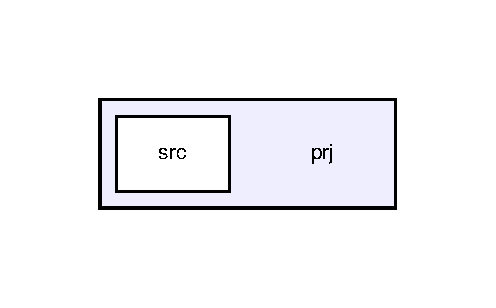
\includegraphics[width=238pt]{dir_7cbe5d391e6e770789076a5282468f8c_dep}
\end{center}
\end{figure}
\subsection*{\-Katalogi}
\begin{DoxyCompactItemize}
\item 
katalog \hyperlink{dir_8a95aa72705647e73a00f13561845afa}{src}
\end{DoxyCompactItemize}

\hypertarget{dir_8a95aa72705647e73a00f13561845afa}{\section{\-Dokumentacja katalogu prj/src/}
\label{dir_8a95aa72705647e73a00f13561845afa}\index{\-Dokumentacja katalogu prj/src/@{\-Dokumentacja katalogu prj/src/}}
}
\-Directory dependency graph for prj/src/\-:\nopagebreak
\begin{figure}[H]
\begin{center}
\leavevmode
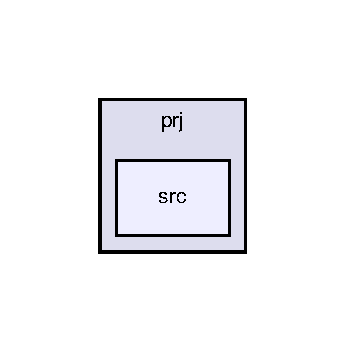
\includegraphics[width=166pt]{dir_8a95aa72705647e73a00f13561845afa_dep}
\end{center}
\end{figure}
\subsection*{\-Pliki}
\begin{DoxyCompactItemize}
\item 
plik \hyperlink{clasa_8cpp}{clasa.\-cpp}
\item 
plik \hyperlink{clasa_8hh}{clasa.\-hh}
\item 
plik \hyperlink{funkcje_8cpp}{funkcje.\-cpp}
\item 
plik \hyperlink{funkcje_8hh}{funkcje.\-hh}
\item 
plik \hyperlink{generator_8cpp}{generator.\-cpp}
\item 
plik \hyperlink{generator_8hh}{generator.\-hh}
\item 
plik \hyperlink{heap_8cpp}{heap.\-cpp}
\item 
plik \hyperlink{heap_8hh}{heap.\-hh}
\item 
plik \hyperlink{main_8cpp}{main.\-cpp}
\item 
plik \hyperlink{merge_8cpp}{merge.\-cpp}
\item 
plik \hyperlink{merge_8hh}{merge.\-hh}
\item 
plik \hyperlink{quick_8cpp}{quick.\-cpp}
\item 
plik \hyperlink{quick_8hh}{quick.\-hh}
\item 
plik \hyperlink{stoper_8hh}{stoper.\-hh}
\end{DoxyCompactItemize}

\chapter{\-Dokumentacja klas}
\hypertarget{classczas}{\section{\-Dokumentacja klasy czas}
\label{classczas}\index{czas@{czas}}
}


{\ttfamily \#include $<$stoper.\-hh$>$}

\subsection*{\-Metody publiczne}
\begin{DoxyCompactItemize}
\item 
void \hyperlink{classczas_a1e4c793526806f459e7f5c8c4a3ae29f}{start} ()
\begin{DoxyCompactList}\small\item\em start pomiaru zapisuje stan zegara \end{DoxyCompactList}\item 
void \hyperlink{classczas_a27f391e3c6bfb1f15f97c61bf403eb2d}{stop} ()
\begin{DoxyCompactList}\small\item\em koniec pomiaru zapisuje stan zegara \end{DoxyCompactList}\item 
double \hyperlink{classczas_a253df7797ca3cc3447d24c3c9477768e}{wynik} ()
\begin{DoxyCompactList}\small\item\em zwraca wynik pomiaru \end{DoxyCompactList}\item 
void \hyperlink{classczas_a53e5d67a7dd77239f2ef6ae0866e0596}{zapisz} (fstream \&\hyperlink{classczas_a253df7797ca3cc3447d24c3c9477768e}{wynik}, int rozmiar)
\begin{DoxyCompactList}\small\item\em zapisuje wynik do pliku \end{DoxyCompactList}\end{DoxyCompactItemize}
\subsection*{\-Atrybuty prywatne}
\begin{DoxyCompactItemize}
\item 
double \hyperlink{classczas_a1348fd4948270410b3087bb0318bd147}{time}
\item 
clock\-\_\-t \hyperlink{classczas_a3e75d47bf9beee497b56997b0b7be45c}{poczatek}
\item 
clock\-\_\-t \hyperlink{classczas_a65324dff284c101f2594b0b05b30399e}{koniec}
\end{DoxyCompactItemize}


\subsection{\-Opis szczegółowy}


\-Definicja w linii 19 pliku stoper.\-hh.



\subsection{\-Dokumentacja funkcji składowych}
\hypertarget{classczas_a1e4c793526806f459e7f5c8c4a3ae29f}{\index{czas@{czas}!start@{start}}
\index{start@{start}!czas@{czas}}
\subsubsection[{start}]{\setlength{\rightskip}{0pt plus 5cm}void {\bf czas\-::start} (
\begin{DoxyParamCaption}
{}
\end{DoxyParamCaption}
)\hspace{0.3cm}{\ttfamily  \mbox{[}inline\mbox{]}}}}\label{classczas_a1e4c793526806f459e7f5c8c4a3ae29f}


start pomiaru zapisuje stan zegara 



\-Definicja w linii 30 pliku stoper.\-hh.



\-Oto graf wywoływań tej funkcji\-:\nopagebreak
\begin{figure}[H]
\begin{center}
\leavevmode
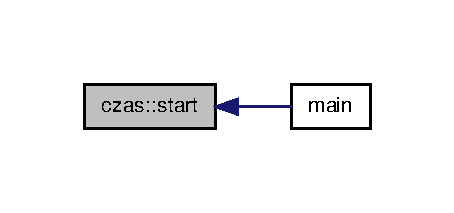
\includegraphics[width=218pt]{classczas_a1e4c793526806f459e7f5c8c4a3ae29f_icgraph}
\end{center}
\end{figure}


\hypertarget{classczas_a27f391e3c6bfb1f15f97c61bf403eb2d}{\index{czas@{czas}!stop@{stop}}
\index{stop@{stop}!czas@{czas}}
\subsubsection[{stop}]{\setlength{\rightskip}{0pt plus 5cm}void {\bf czas\-::stop} (
\begin{DoxyParamCaption}
{}
\end{DoxyParamCaption}
)\hspace{0.3cm}{\ttfamily  \mbox{[}inline\mbox{]}}}}\label{classczas_a27f391e3c6bfb1f15f97c61bf403eb2d}


koniec pomiaru zapisuje stan zegara 



\-Definicja w linii 38 pliku stoper.\-hh.



\-Oto graf wywoływań tej funkcji\-:\nopagebreak
\begin{figure}[H]
\begin{center}
\leavevmode
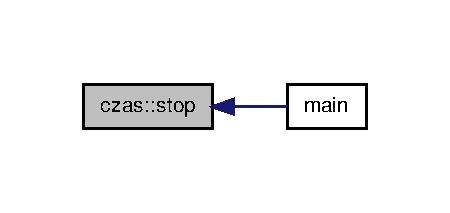
\includegraphics[width=216pt]{classczas_a27f391e3c6bfb1f15f97c61bf403eb2d_icgraph}
\end{center}
\end{figure}


\hypertarget{classczas_a253df7797ca3cc3447d24c3c9477768e}{\index{czas@{czas}!wynik@{wynik}}
\index{wynik@{wynik}!czas@{czas}}
\subsubsection[{wynik}]{\setlength{\rightskip}{0pt plus 5cm}double {\bf czas\-::wynik} (
\begin{DoxyParamCaption}
{}
\end{DoxyParamCaption}
)\hspace{0.3cm}{\ttfamily  \mbox{[}inline\mbox{]}}}}\label{classczas_a253df7797ca3cc3447d24c3c9477768e}


zwraca wynik pomiaru 

\begin{DoxyReturn}{\-Zwraca}
zwraca czas dzialania 
\end{DoxyReturn}


\-Definicja w linii 46 pliku stoper.\-hh.



\-Oto graf wywoływań tej funkcji\-:\nopagebreak
\begin{figure}[H]
\begin{center}
\leavevmode
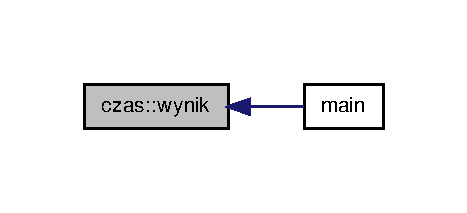
\includegraphics[width=224pt]{classczas_a253df7797ca3cc3447d24c3c9477768e_icgraph}
\end{center}
\end{figure}


\hypertarget{classczas_a53e5d67a7dd77239f2ef6ae0866e0596}{\index{czas@{czas}!zapisz@{zapisz}}
\index{zapisz@{zapisz}!czas@{czas}}
\subsubsection[{zapisz}]{\setlength{\rightskip}{0pt plus 5cm}void {\bf czas\-::zapisz} (
\begin{DoxyParamCaption}
\item[{fstream \&}]{wynik, }
\item[{int}]{rozmiar}
\end{DoxyParamCaption}
)\hspace{0.3cm}{\ttfamily  \mbox{[}inline\mbox{]}}}}\label{classczas_a53e5d67a7dd77239f2ef6ae0866e0596}


zapisuje wynik do pliku 


\begin{DoxyParams}{\-Parametry}
{\em wynik} & pomiaru \\
\hline
{\em rozmiar} & rozmiar problemu \\
\hline
\end{DoxyParams}


\-Definicja w linii 56 pliku stoper.\-hh.



\subsection{\-Dokumentacja atrybutów składowych}
\hypertarget{classczas_a65324dff284c101f2594b0b05b30399e}{\index{czas@{czas}!koniec@{koniec}}
\index{koniec@{koniec}!czas@{czas}}
\subsubsection[{koniec}]{\setlength{\rightskip}{0pt plus 5cm}clock\-\_\-t {\bf czas\-::koniec}\hspace{0.3cm}{\ttfamily  \mbox{[}private\mbox{]}}}}\label{classczas_a65324dff284c101f2594b0b05b30399e}


\-Definicja w linii 24 pliku stoper.\-hh.

\hypertarget{classczas_a3e75d47bf9beee497b56997b0b7be45c}{\index{czas@{czas}!poczatek@{poczatek}}
\index{poczatek@{poczatek}!czas@{czas}}
\subsubsection[{poczatek}]{\setlength{\rightskip}{0pt plus 5cm}clock\-\_\-t {\bf czas\-::poczatek}\hspace{0.3cm}{\ttfamily  \mbox{[}private\mbox{]}}}}\label{classczas_a3e75d47bf9beee497b56997b0b7be45c}


\-Definicja w linii 24 pliku stoper.\-hh.

\hypertarget{classczas_a1348fd4948270410b3087bb0318bd147}{\index{czas@{czas}!time@{time}}
\index{time@{time}!czas@{czas}}
\subsubsection[{time}]{\setlength{\rightskip}{0pt plus 5cm}double {\bf czas\-::time}\hspace{0.3cm}{\ttfamily  \mbox{[}private\mbox{]}}}}\label{classczas_a1348fd4948270410b3087bb0318bd147}


\-Definicja w linii 23 pliku stoper.\-hh.



\-Dokumentacja dla tej klasy została wygenerowana z pliku\-:\begin{DoxyCompactItemize}
\item 
\hyperlink{stoper_8hh}{stoper.\-hh}\end{DoxyCompactItemize}

\hypertarget{classdane}{\section{\-Dokumentacja klasy dane}
\label{classdane}\index{dane@{dane}}
}


{\ttfamily \#include $<$clasa.\-hh$>$}

\subsection*{\-Metody publiczne}
\begin{DoxyCompactItemize}
\item 
bool \hyperlink{classdane_a09b0fdc6cf2fa99c6c2f68d4c0030744}{\-Zamien\-\_\-elementy} (int a, int b)
\begin{DoxyCompactList}\small\item\em funkcja zamienia elementy o podanym indexie \end{DoxyCompactList}\item 
void \hyperlink{classdane_ae749fc29f90e1319e2ce90ad4468c493}{odwroc} ()
\begin{DoxyCompactList}\small\item\em funkcja kolejnosc wystepowania elementow \end{DoxyCompactList}\item 
bool \hyperlink{classdane_a5e78dfce6c067184fcab87fc240c1aae}{dodaj} (int element, int miejsce)
\begin{DoxyCompactList}\small\item\em funkcja dodaje element we wskazane miejsce \end{DoxyCompactList}\item 
void \hyperlink{classdane_a7bcc9aec78734af1ee645dc9ebe1287b}{dodaj\-\_\-koniec} (int element)
\begin{DoxyCompactList}\small\item\em dodaje element na koniec wektora \end{DoxyCompactList}\item 
void \hyperlink{classdane_ad44c49c93a1eae29da38e0392a45f44d}{dodaj\-\_\-poczatek} (int element)
\begin{DoxyCompactList}\small\item\em dodaje element na poczatek \end{DoxyCompactList}\item 
bool \hyperlink{classdane_aff5590550b2314aad3112910d8d53a26}{dodaj} (int $\ast$tab, int ilosc, int miejsce)
\begin{DoxyCompactList}\small\item\em dodaje tablice elementow \end{DoxyCompactList}\item 
bool \hyperlink{classdane_a110ef86ae677f7c30860dcc4f935e35f}{operator==} (vector$<$ int $>$ wektor)
\begin{DoxyCompactList}\small\item\em porownuje vektor zewnetrzny z wektorem klasy \end{DoxyCompactList}\item 
void \hyperlink{classdane_a058ddbd9e4776c8d46310c67ba22c6db}{operator+} (vector$<$ int $>$ element)
\begin{DoxyCompactList}\small\item\em dodaje vektor do vektora w klasie \end{DoxyCompactList}\item 
bool \hyperlink{classdane_ab2387c22ea50d971126631d094f48376}{operator==} (\hyperlink{classdane}{dane} drugi)
\begin{DoxyCompactList}\small\item\em porownuje dwie klasy dane \end{DoxyCompactList}\end{DoxyCompactItemize}
\subsection*{\-Atrybuty publiczne}
\begin{DoxyCompactItemize}
\item 
vector$<$ int $>$ \hyperlink{classdane_a54607ce56b0cf755637110b0b81f5dde}{wejsciowe}
\item 
int \hyperlink{classdane_ac22495cbe79aa41bf0d6c44a27755306}{rozmiar}
\end{DoxyCompactItemize}
\subsection*{\-Przyjaciele}
\begin{DoxyCompactItemize}
\item 
ostream \& \hyperlink{classdane_a7ed2c8398056f86ea981b02c3abe3a1f}{operator$<$$<$} (ostream \&wyjscie, \hyperlink{classdane}{dane} \&wej)
\item 
fstream \& \hyperlink{classdane_a4f5402546464f59b7fdf3a9a5e5be220}{operator$>$$>$} (fstream \&plik, \hyperlink{classdane}{dane} \&wej)
\end{DoxyCompactItemize}


\subsection{\-Opis szczegółowy}


\-Definicja w linii 14 pliku clasa.\-hh.



\subsection{\-Dokumentacja funkcji składowych}
\hypertarget{classdane_a5e78dfce6c067184fcab87fc240c1aae}{\index{dane@{dane}!dodaj@{dodaj}}
\index{dodaj@{dodaj}!dane@{dane}}
\subsubsection[{dodaj}]{\setlength{\rightskip}{0pt plus 5cm}bool {\bf dane\-::dodaj} (
\begin{DoxyParamCaption}
\item[{int}]{element, }
\item[{int}]{miejsce}
\end{DoxyParamCaption}
)}}\label{classdane_a5e78dfce6c067184fcab87fc240c1aae}


funkcja dodaje element we wskazane miejsce 


\begin{DoxyParams}{\-Parametry}
{\em element} & ktory ma zostac wstawiony \\
\hline
{\em miejsce} & w ktore ma zostac wstawiony element \\
\hline
\end{DoxyParams}
\begin{DoxyReturn}{\-Zwraca}
zwraca false jesli index jest zbyt duzy 
\end{DoxyReturn}


\-Definicja w linii 45 pliku clasa.\-cpp.

\hypertarget{classdane_aff5590550b2314aad3112910d8d53a26}{\index{dane@{dane}!dodaj@{dodaj}}
\index{dodaj@{dodaj}!dane@{dane}}
\subsubsection[{dodaj}]{\setlength{\rightskip}{0pt plus 5cm}bool {\bf dane\-::dodaj} (
\begin{DoxyParamCaption}
\item[{int $\ast$}]{tab, }
\item[{int}]{ilosc, }
\item[{int}]{miejsce}
\end{DoxyParamCaption}
)}}\label{classdane_aff5590550b2314aad3112910d8d53a26}


dodaje tablice elementow 

elementy sa dodawane we wskazane miejsce indeksujemy od 1 
\begin{DoxyParams}{\-Parametry}
{\em tab} & wskaznik na tablice elementow \\
\hline
{\em ilosc} & elementow do dodania \\
\hline
{\em miejsce} & index miejsca w ktore ma zostawc wstawiona tablica \\
\hline
\end{DoxyParams}
\begin{DoxyReturn}{\-Zwraca}

\end{DoxyReturn}


\-Definicja w linii 82 pliku clasa.\-cpp.

\hypertarget{classdane_a7bcc9aec78734af1ee645dc9ebe1287b}{\index{dane@{dane}!dodaj\-\_\-koniec@{dodaj\-\_\-koniec}}
\index{dodaj\-\_\-koniec@{dodaj\-\_\-koniec}!dane@{dane}}
\subsubsection[{dodaj\-\_\-koniec}]{\setlength{\rightskip}{0pt plus 5cm}void {\bf dane\-::dodaj\-\_\-koniec} (
\begin{DoxyParamCaption}
\item[{int}]{element}
\end{DoxyParamCaption}
)}}\label{classdane_a7bcc9aec78734af1ee645dc9ebe1287b}


dodaje element na koniec wektora 


\begin{DoxyParams}{\-Parametry}
{\em element} & ktory ma zostac dodany \\
\hline
\end{DoxyParams}


\-Definicja w linii 58 pliku clasa.\-cpp.

\hypertarget{classdane_ad44c49c93a1eae29da38e0392a45f44d}{\index{dane@{dane}!dodaj\-\_\-poczatek@{dodaj\-\_\-poczatek}}
\index{dodaj\-\_\-poczatek@{dodaj\-\_\-poczatek}!dane@{dane}}
\subsubsection[{dodaj\-\_\-poczatek}]{\setlength{\rightskip}{0pt plus 5cm}void {\bf dane\-::dodaj\-\_\-poczatek} (
\begin{DoxyParamCaption}
\item[{int}]{element}
\end{DoxyParamCaption}
)}}\label{classdane_ad44c49c93a1eae29da38e0392a45f44d}


dodaje element na poczatek 


\begin{DoxyParams}{\-Parametry}
{\em element} & ktory ma zostac dodany \\
\hline
\end{DoxyParams}


\-Definicja w linii 67 pliku clasa.\-cpp.

\hypertarget{classdane_ae749fc29f90e1319e2ce90ad4468c493}{\index{dane@{dane}!odwroc@{odwroc}}
\index{odwroc@{odwroc}!dane@{dane}}
\subsubsection[{odwroc}]{\setlength{\rightskip}{0pt plus 5cm}void {\bf dane\-::odwroc} (
\begin{DoxyParamCaption}
{}
\end{DoxyParamCaption}
)}}\label{classdane_ae749fc29f90e1319e2ce90ad4468c493}


funkcja kolejnosc wystepowania elementow 



\-Definicja w linii 31 pliku clasa.\-cpp.



\-Oto graf wywołań dla tej funkcji\-:\nopagebreak
\begin{figure}[H]
\begin{center}
\leavevmode
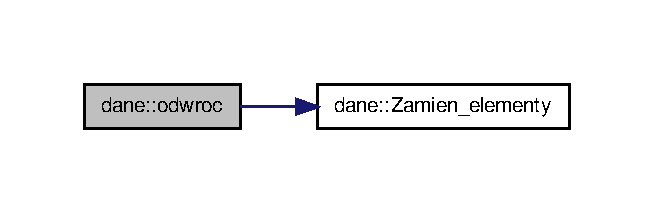
\includegraphics[width=314pt]{classdane_ae749fc29f90e1319e2ce90ad4468c493_cgraph}
\end{center}
\end{figure}


\hypertarget{classdane_a058ddbd9e4776c8d46310c67ba22c6db}{\index{dane@{dane}!operator+@{operator+}}
\index{operator+@{operator+}!dane@{dane}}
\subsubsection[{operator+}]{\setlength{\rightskip}{0pt plus 5cm}void dane\-::operator+ (
\begin{DoxyParamCaption}
\item[{vector$<$ int $>$}]{element}
\end{DoxyParamCaption}
)}}\label{classdane_a058ddbd9e4776c8d46310c67ba22c6db}


dodaje vektor do vektora w klasie 


\begin{DoxyParams}{\-Parametry}
{\em element} & vektor ktory ma zostac dodany \\
\hline
\end{DoxyParams}


\-Definicja w linii 112 pliku clasa.\-cpp.

\hypertarget{classdane_a110ef86ae677f7c30860dcc4f935e35f}{\index{dane@{dane}!operator==@{operator==}}
\index{operator==@{operator==}!dane@{dane}}
\subsubsection[{operator==}]{\setlength{\rightskip}{0pt plus 5cm}bool dane\-::operator== (
\begin{DoxyParamCaption}
\item[{vector$<$ int $>$}]{wektor}
\end{DoxyParamCaption}
)}}\label{classdane_a110ef86ae677f7c30860dcc4f935e35f}


porownuje vektor zewnetrzny z wektorem klasy 


\begin{DoxyParams}{\-Parametry}
{\em wektor} & zewnetrzny \\
\hline
\end{DoxyParams}
\begin{DoxyReturn}{\-Zwraca}

\end{DoxyReturn}


\-Definicja w linii 99 pliku clasa.\-cpp.

\hypertarget{classdane_ab2387c22ea50d971126631d094f48376}{\index{dane@{dane}!operator==@{operator==}}
\index{operator==@{operator==}!dane@{dane}}
\subsubsection[{operator==}]{\setlength{\rightskip}{0pt plus 5cm}bool dane\-::operator== (
\begin{DoxyParamCaption}
\item[{{\bf dane}}]{drugi}
\end{DoxyParamCaption}
)}}\label{classdane_ab2387c22ea50d971126631d094f48376}


porownuje dwie klasy dane 


\begin{DoxyParams}{\-Parametry}
{\em drugi} & \\
\hline
\end{DoxyParams}
\begin{DoxyReturn}{\-Zwraca}

\end{DoxyReturn}


\-Definicja w linii 130 pliku clasa.\-cpp.

\hypertarget{classdane_a09b0fdc6cf2fa99c6c2f68d4c0030744}{\index{dane@{dane}!\-Zamien\-\_\-elementy@{\-Zamien\-\_\-elementy}}
\index{\-Zamien\-\_\-elementy@{\-Zamien\-\_\-elementy}!dane@{dane}}
\subsubsection[{\-Zamien\-\_\-elementy}]{\setlength{\rightskip}{0pt plus 5cm}bool {\bf dane\-::\-Zamien\-\_\-elementy} (
\begin{DoxyParamCaption}
\item[{int}]{a, }
\item[{int}]{b}
\end{DoxyParamCaption}
)}}\label{classdane_a09b0fdc6cf2fa99c6c2f68d4c0030744}


funkcja zamienia elementy o podanym indexie 

elementy indexowane sa od 0, 
\begin{DoxyParams}{\-Parametry}
{\em a} & element pierwszy \\
\hline
{\em b} & element drugi \\
\hline
\end{DoxyParams}
\begin{DoxyReturn}{\-Zwraca}
zwraca false jesli index jest zbyt duzy 
\end{DoxyReturn}


\-Definicja w linii 16 pliku clasa.\-cpp.



\-Oto graf wywoływań tej funkcji\-:\nopagebreak
\begin{figure}[H]
\begin{center}
\leavevmode
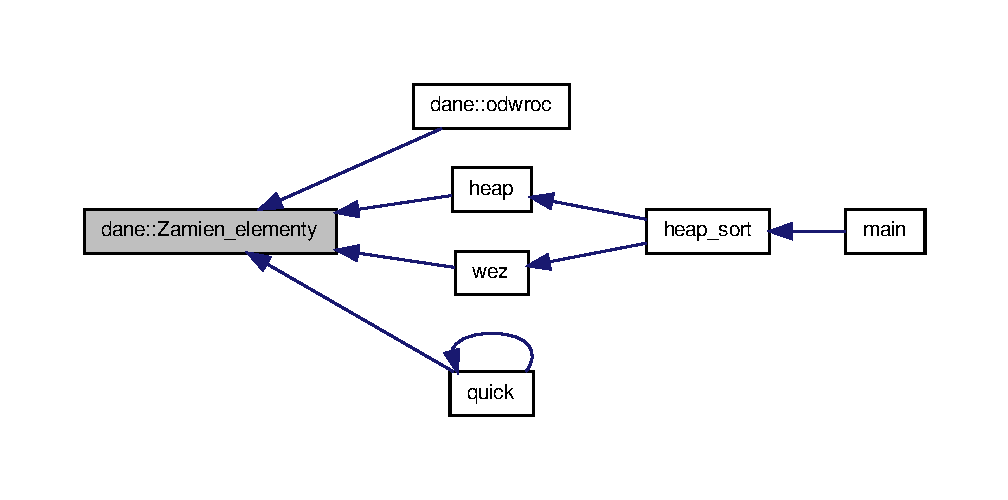
\includegraphics[width=350pt]{classdane_a09b0fdc6cf2fa99c6c2f68d4c0030744_icgraph}
\end{center}
\end{figure}




\subsection{\-Dokumentacja przyjaciół i funkcji związanych}
\hypertarget{classdane_a7ed2c8398056f86ea981b02c3abe3a1f}{\index{dane@{dane}!operator$<$$<$@{operator$<$$<$}}
\index{operator$<$$<$@{operator$<$$<$}!dane@{dane}}
\subsubsection[{operator$<$$<$}]{\setlength{\rightskip}{0pt plus 5cm}ostream\& operator$<$$<$ (
\begin{DoxyParamCaption}
\item[{ostream \&}]{wyjscie, }
\item[{{\bf dane} \&}]{wej}
\end{DoxyParamCaption}
)\hspace{0.3cm}{\ttfamily  \mbox{[}friend\mbox{]}}}}\label{classdane_a7ed2c8398056f86ea981b02c3abe3a1f}


\-Definicja w linii 20 pliku clasa.\-hh.

\hypertarget{classdane_a4f5402546464f59b7fdf3a9a5e5be220}{\index{dane@{dane}!operator$>$$>$@{operator$>$$>$}}
\index{operator$>$$>$@{operator$>$$>$}!dane@{dane}}
\subsubsection[{operator$>$$>$}]{\setlength{\rightskip}{0pt plus 5cm}fstream\& operator$>$$>$ (
\begin{DoxyParamCaption}
\item[{fstream \&}]{plik, }
\item[{{\bf dane} \&}]{wej}
\end{DoxyParamCaption}
)\hspace{0.3cm}{\ttfamily  \mbox{[}friend\mbox{]}}}}\label{classdane_a4f5402546464f59b7fdf3a9a5e5be220}


\-Definicja w linii 30 pliku clasa.\-hh.



\subsection{\-Dokumentacja atrybutów składowych}
\hypertarget{classdane_ac22495cbe79aa41bf0d6c44a27755306}{\index{dane@{dane}!rozmiar@{rozmiar}}
\index{rozmiar@{rozmiar}!dane@{dane}}
\subsubsection[{rozmiar}]{\setlength{\rightskip}{0pt plus 5cm}int {\bf dane\-::rozmiar}}}\label{classdane_ac22495cbe79aa41bf0d6c44a27755306}


\-Definicja w linii 18 pliku clasa.\-hh.

\hypertarget{classdane_a54607ce56b0cf755637110b0b81f5dde}{\index{dane@{dane}!wejsciowe@{wejsciowe}}
\index{wejsciowe@{wejsciowe}!dane@{dane}}
\subsubsection[{wejsciowe}]{\setlength{\rightskip}{0pt plus 5cm}vector$<$int$>$ {\bf dane\-::wejsciowe}}}\label{classdane_a54607ce56b0cf755637110b0b81f5dde}


\-Definicja w linii 17 pliku clasa.\-hh.



\-Dokumentacja dla tej klasy została wygenerowana z plików\-:\begin{DoxyCompactItemize}
\item 
\hyperlink{clasa_8hh}{clasa.\-hh}\item 
\hyperlink{clasa_8cpp}{clasa.\-cpp}\end{DoxyCompactItemize}

\chapter{\-Dokumentacja plików}
\hypertarget{clasa_8cpp}{\section{\-Dokumentacja pliku clasa.\-cpp}
\label{clasa_8cpp}\index{clasa.\-cpp@{clasa.\-cpp}}
}
{\ttfamily \#include \char`\"{}clasa.\-hh\char`\"{}}\*
\-Wykres zależności załączania dla clasa.\-cpp\-:\nopagebreak
\begin{figure}[H]
\begin{center}
\leavevmode
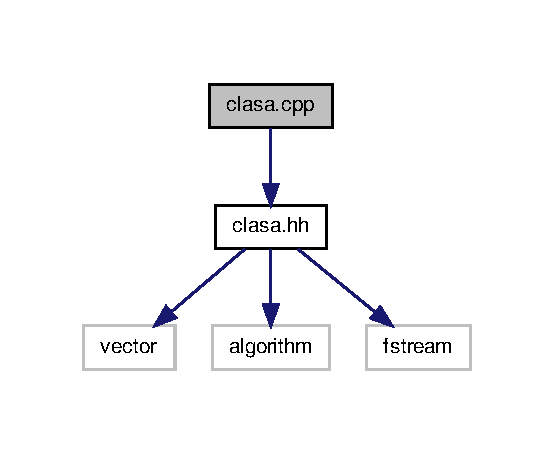
\includegraphics[width=266pt]{clasa_8cpp__incl}
\end{center}
\end{figure}

\hypertarget{clasa_8hh}{\section{\-Dokumentacja pliku clasa.\-hh}
\label{clasa_8hh}\index{clasa.\-hh@{clasa.\-hh}}
}
{\ttfamily \#include $<$vector$>$}\*
{\ttfamily \#include $<$algorithm$>$}\*
{\ttfamily \#include $<$fstream$>$}\*
\-Wykres zależności załączania dla clasa.\-hh\-:\nopagebreak
\begin{figure}[H]
\begin{center}
\leavevmode
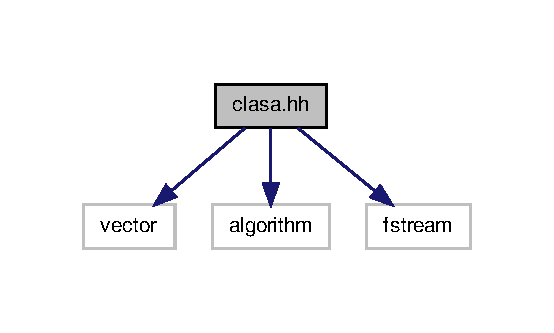
\includegraphics[width=266pt]{clasa_8hh__incl}
\end{center}
\end{figure}
\-Ten wykres pokazuje, które pliki bezpośrednio lub pośrednio załączają ten plik\-:\nopagebreak
\begin{figure}[H]
\begin{center}
\leavevmode
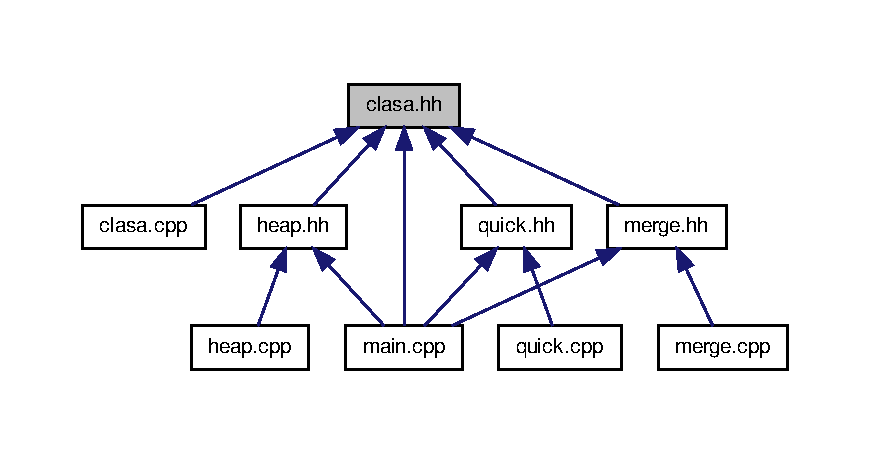
\includegraphics[width=350pt]{clasa_8hh__dep__incl}
\end{center}
\end{figure}
\subsection*{\-Komponenty}
\begin{DoxyCompactItemize}
\item 
class \hyperlink{classdane}{dane}
\end{DoxyCompactItemize}

\hypertarget{funkcje_8cpp}{\section{\-Dokumentacja pliku funkcje.\-cpp}
\label{funkcje_8cpp}\index{funkcje.\-cpp@{funkcje.\-cpp}}
}
{\ttfamily \#include \char`\"{}funkcje.\-hh\char`\"{}}\*
\-Wykres zależności załączania dla funkcje.\-cpp\-:\nopagebreak
\begin{figure}[H]
\begin{center}
\leavevmode
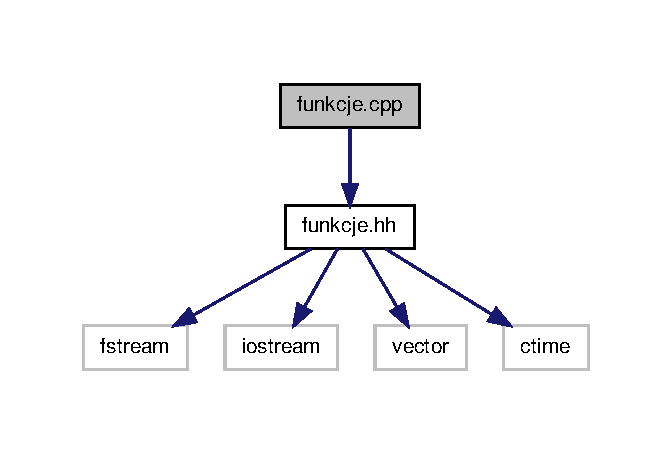
\includegraphics[width=322pt]{funkcje_8cpp__incl}
\end{center}
\end{figure}
\subsection*{\-Funkcje}
\begin{DoxyCompactItemize}
\item 
bool \hyperlink{funkcje_8cpp_ab80d311fc13e71453f3080482634447e}{otworz} (char $\ast$nazwa, fstream \&plik)
\begin{DoxyCompactList}\small\item\em otwiera plik o zadajnej nazwie \end{DoxyCompactList}\item 
int \hyperlink{funkcje_8cpp_a1cddff5e49afc682449b3bda713006f5}{kopiuj} (vector$<$ int $>$ \&wejsciowe, fstream \&plik)
\begin{DoxyCompactList}\small\item\em kopiuje dane z pliku do wektora \end{DoxyCompactList}\item 
double \hyperlink{funkcje_8cpp_ad9ebe61e239dee170b242bda4db9ea63}{obliczenia} (const vector$<$ int $>$ \&wejsciowe, int $\ast$wyjsciowe, int powt)
\begin{DoxyCompactList}\small\item\em implementacja pomiatu czasu oraz algorytmu mnozenia \end{DoxyCompactList}\item 
void \hyperlink{funkcje_8cpp_aaa6c62fc60fb1173b904269379d69754}{zapisz} (int $\ast$tablica, fstream \&plik, int rozmiar)
\begin{DoxyCompactList}\small\item\em funkcja kopiuje zawartosc tablicy wynikow do pliku \end{DoxyCompactList}\end{DoxyCompactItemize}


\subsection{\-Dokumentacja funkcji}
\hypertarget{funkcje_8cpp_a1cddff5e49afc682449b3bda713006f5}{\index{funkcje.\-cpp@{funkcje.\-cpp}!kopiuj@{kopiuj}}
\index{kopiuj@{kopiuj}!funkcje.cpp@{funkcje.\-cpp}}
\subsubsection[{kopiuj}]{\setlength{\rightskip}{0pt plus 5cm}int {\bf kopiuj} (
\begin{DoxyParamCaption}
\item[{vector$<$ int $>$ \&}]{wejsciowe, }
\item[{fstream \&}]{plik}
\end{DoxyParamCaption}
)}}\label{funkcje_8cpp_a1cddff5e49afc682449b3bda713006f5}


kopiuje dane z pliku do wektora 

\-Funkcja pobiera wiersz danych z strumienia wejsciwego i zapisuje go w postaci zmiennej int do wektora 
\begin{DoxyParams}{\-Parametry}
{\em wejsciowe} & referencja wekstora przechowywujacego dane wejsciowe \\
\hline
{\em plik} & strumien wejscia zachaczony na pliku z danymi wejsciowymi \\
\hline
\end{DoxyParams}
\begin{DoxyReturn}{\-Zwraca}
zwraca rozmiar tablic 
\end{DoxyReturn}


\-Definicja w linii 32 pliku funkcje.\-cpp.

\hypertarget{funkcje_8cpp_ad9ebe61e239dee170b242bda4db9ea63}{\index{funkcje.\-cpp@{funkcje.\-cpp}!obliczenia@{obliczenia}}
\index{obliczenia@{obliczenia}!funkcje.cpp@{funkcje.\-cpp}}
\subsubsection[{obliczenia}]{\setlength{\rightskip}{0pt plus 5cm}double {\bf obliczenia} (
\begin{DoxyParamCaption}
\item[{const vector$<$ int $>$ \&}]{wejsciowe, }
\item[{int $\ast$}]{wyjsciowe, }
\item[{int}]{powt}
\end{DoxyParamCaption}
)}}\label{funkcje_8cpp_ad9ebe61e239dee170b242bda4db9ea63}


implementacja pomiatu czasu oraz algorytmu mnozenia 

w fuknkcji zostaje zmierzona ilość taktów procesora potrzebnych na wykonanie

zadanej ilości opercji mnożenia. \-Następnie ilość taktów zostaje podzielona przez

stała \-P\-E\-R\-\_\-\-T\-O\-\_\-\-S\-E\-C 
\begin{DoxyParams}{\-Parametry}
{\em wejsciowe} & dane ktore przetworzy algorytm \\
\hline
{\em wyjsciowe} & tablica wynikow mnozenia \\
\hline
{\em powt} & liczba powtorzen algorytmu \\
\hline
\end{DoxyParams}


\-Definicja w linii 54 pliku funkcje.\-cpp.

\hypertarget{funkcje_8cpp_ab80d311fc13e71453f3080482634447e}{\index{funkcje.\-cpp@{funkcje.\-cpp}!otworz@{otworz}}
\index{otworz@{otworz}!funkcje.cpp@{funkcje.\-cpp}}
\subsubsection[{otworz}]{\setlength{\rightskip}{0pt plus 5cm}bool {\bf otworz} (
\begin{DoxyParamCaption}
\item[{char $\ast$}]{nazwa, }
\item[{fstream \&}]{plik}
\end{DoxyParamCaption}
)}}\label{funkcje_8cpp_ab80d311fc13e71453f3080482634447e}


otwiera plik o zadajnej nazwie 


\begin{DoxyParams}{\-Parametry}
{\em nazwa} & sciezka do pliku \\
\hline
{\em plik} & uchwyt do pliku \\
\hline
\end{DoxyParams}
\begin{DoxyReturn}{\-Zwraca}

\end{DoxyReturn}


\-Definicja w linii 18 pliku funkcje.\-cpp.

\hypertarget{funkcje_8cpp_aaa6c62fc60fb1173b904269379d69754}{\index{funkcje.\-cpp@{funkcje.\-cpp}!zapisz@{zapisz}}
\index{zapisz@{zapisz}!funkcje.cpp@{funkcje.\-cpp}}
\subsubsection[{zapisz}]{\setlength{\rightskip}{0pt plus 5cm}void {\bf zapisz} (
\begin{DoxyParamCaption}
\item[{int $\ast$}]{tablica, }
\item[{fstream \&}]{plik, }
\item[{int}]{rozmiar}
\end{DoxyParamCaption}
)}}\label{funkcje_8cpp_aaa6c62fc60fb1173b904269379d69754}


funkcja kopiuje zawartosc tablicy wynikow do pliku 


\begin{DoxyParams}{\-Parametry}
{\em tablica} & \\
\hline
{\em plik} & \\
\hline
{\em rozmiar} & \\
\hline
\end{DoxyParams}


\-Definicja w linii 87 pliku funkcje.\-cpp.


\hypertarget{funkcje_8hh}{\section{\-Dokumentacja pliku funkcje.\-hh}
\label{funkcje_8hh}\index{funkcje.\-hh@{funkcje.\-hh}}
}
{\ttfamily \#include $<$fstream$>$}\*
{\ttfamily \#include $<$iostream$>$}\*
{\ttfamily \#include $<$vector$>$}\*
{\ttfamily \#include $<$ctime$>$}\*
\-Wykres zależności załączania dla funkcje.\-hh\-:\nopagebreak
\begin{figure}[H]
\begin{center}
\leavevmode
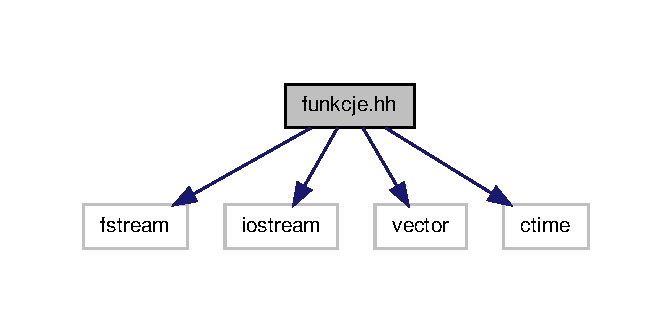
\includegraphics[width=322pt]{funkcje_8hh__incl}
\end{center}
\end{figure}
\-Ten wykres pokazuje, które pliki bezpośrednio lub pośrednio załączają ten plik\-:\nopagebreak
\begin{figure}[H]
\begin{center}
\leavevmode
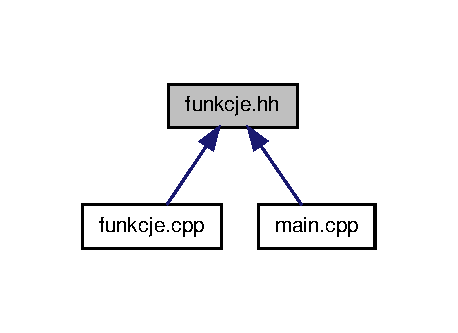
\includegraphics[width=220pt]{funkcje_8hh__dep__incl}
\end{center}
\end{figure}
\subsection*{\-Definicje}
\begin{DoxyCompactItemize}
\item 
\#define \hyperlink{funkcje_8hh_a3d9fc3c745d0880902fe3ea3d5d5f71e}{\-C\-L\-O\-C\-K\-S\-\_\-\-P\-E\-R\-\_\-\-S\-E\-C}~1000000
\end{DoxyCompactItemize}
\subsection*{\-Funkcje}
\begin{DoxyCompactItemize}
\item 
void \hyperlink{funkcje_8hh_aaa6c62fc60fb1173b904269379d69754}{zapisz} (int $\ast$tablica, fstream \&plik, int rozmiar)
\begin{DoxyCompactList}\small\item\em funkcja kopiuje zawartosc tablicy wynikow do pliku \end{DoxyCompactList}\item 
double \hyperlink{funkcje_8hh_ad9ebe61e239dee170b242bda4db9ea63}{obliczenia} (const vector$<$ int $>$ \&wejsciowe, int $\ast$wyjsciowe, int powt)
\begin{DoxyCompactList}\small\item\em implementacja pomiatu czasu oraz algorytmu mnozenia \end{DoxyCompactList}\item 
bool \hyperlink{funkcje_8hh_ab80d311fc13e71453f3080482634447e}{otworz} (char $\ast$nazwa, fstream \&plik)
\begin{DoxyCompactList}\small\item\em otwiera plik o zadajnej nazwie \end{DoxyCompactList}\item 
int \hyperlink{funkcje_8hh_a1cddff5e49afc682449b3bda713006f5}{kopiuj} (vector$<$ int $>$ \&wejsciowe, fstream \&plik)
\begin{DoxyCompactList}\small\item\em kopiuje dane z pliku do wektora \end{DoxyCompactList}\end{DoxyCompactItemize}


\subsection{\-Dokumentacja definicji}
\hypertarget{funkcje_8hh_a3d9fc3c745d0880902fe3ea3d5d5f71e}{\index{funkcje.\-hh@{funkcje.\-hh}!\-C\-L\-O\-C\-K\-S\-\_\-\-P\-E\-R\-\_\-\-S\-E\-C@{\-C\-L\-O\-C\-K\-S\-\_\-\-P\-E\-R\-\_\-\-S\-E\-C}}
\index{\-C\-L\-O\-C\-K\-S\-\_\-\-P\-E\-R\-\_\-\-S\-E\-C@{\-C\-L\-O\-C\-K\-S\-\_\-\-P\-E\-R\-\_\-\-S\-E\-C}!funkcje.hh@{funkcje.\-hh}}
\subsubsection[{\-C\-L\-O\-C\-K\-S\-\_\-\-P\-E\-R\-\_\-\-S\-E\-C}]{\setlength{\rightskip}{0pt plus 5cm}\#define {\bf \-C\-L\-O\-C\-K\-S\-\_\-\-P\-E\-R\-\_\-\-S\-E\-C}~1000000}}\label{funkcje_8hh_a3d9fc3c745d0880902fe3ea3d5d5f71e}


\-Definicja w linii 14 pliku funkcje.\-hh.



\subsection{\-Dokumentacja funkcji}
\hypertarget{funkcje_8hh_a1cddff5e49afc682449b3bda713006f5}{\index{funkcje.\-hh@{funkcje.\-hh}!kopiuj@{kopiuj}}
\index{kopiuj@{kopiuj}!funkcje.hh@{funkcje.\-hh}}
\subsubsection[{kopiuj}]{\setlength{\rightskip}{0pt plus 5cm}int {\bf kopiuj} (
\begin{DoxyParamCaption}
\item[{vector$<$ int $>$ \&}]{wejsciowe, }
\item[{fstream \&}]{plik}
\end{DoxyParamCaption}
)}}\label{funkcje_8hh_a1cddff5e49afc682449b3bda713006f5}


kopiuje dane z pliku do wektora 

\-Funkcja pobiera wiersz danych z strumienia wejsciwego i zapisuje go w postaci zmiennej int do wektora 
\begin{DoxyParams}{\-Parametry}
{\em wejsciowe} & referencja wekstora przechowywujacego dane wejsciowe \\
\hline
{\em plik} & strumien wejscia zachaczony na pliku z danymi wejsciowymi \\
\hline
\end{DoxyParams}
\begin{DoxyReturn}{\-Zwraca}
zwraca rozmiar tablic 
\end{DoxyReturn}


\-Definicja w linii 32 pliku funkcje.\-cpp.

\hypertarget{funkcje_8hh_ad9ebe61e239dee170b242bda4db9ea63}{\index{funkcje.\-hh@{funkcje.\-hh}!obliczenia@{obliczenia}}
\index{obliczenia@{obliczenia}!funkcje.hh@{funkcje.\-hh}}
\subsubsection[{obliczenia}]{\setlength{\rightskip}{0pt plus 5cm}double {\bf obliczenia} (
\begin{DoxyParamCaption}
\item[{const vector$<$ int $>$ \&}]{wejsciowe, }
\item[{int $\ast$}]{wyjsciowe, }
\item[{int}]{powt}
\end{DoxyParamCaption}
)}}\label{funkcje_8hh_ad9ebe61e239dee170b242bda4db9ea63}


implementacja pomiatu czasu oraz algorytmu mnozenia 

w fuknkcji zostaje zmierzona ilość taktów procesora potrzebnych na wykonanie

zadanej ilości opercji mnożenia. \-Następnie ilość taktów zostaje podzielona przez

stała \-P\-E\-R\-\_\-\-T\-O\-\_\-\-S\-E\-C 
\begin{DoxyParams}{\-Parametry}
{\em wejsciowe} & dane ktore przetworzy algorytm \\
\hline
{\em wyjsciowe} & tablica wynikow mnozenia \\
\hline
{\em powt} & liczba powtorzen algorytmu \\
\hline
\end{DoxyParams}


\-Definicja w linii 54 pliku funkcje.\-cpp.

\hypertarget{funkcje_8hh_ab80d311fc13e71453f3080482634447e}{\index{funkcje.\-hh@{funkcje.\-hh}!otworz@{otworz}}
\index{otworz@{otworz}!funkcje.hh@{funkcje.\-hh}}
\subsubsection[{otworz}]{\setlength{\rightskip}{0pt plus 5cm}bool {\bf otworz} (
\begin{DoxyParamCaption}
\item[{char $\ast$}]{nazwa, }
\item[{fstream \&}]{plik}
\end{DoxyParamCaption}
)}}\label{funkcje_8hh_ab80d311fc13e71453f3080482634447e}


otwiera plik o zadajnej nazwie 


\begin{DoxyParams}{\-Parametry}
{\em nazwa} & sciezka do pliku \\
\hline
{\em plik} & uchwyt do pliku \\
\hline
\end{DoxyParams}
\begin{DoxyReturn}{\-Zwraca}

\end{DoxyReturn}


\-Definicja w linii 18 pliku funkcje.\-cpp.

\hypertarget{funkcje_8hh_aaa6c62fc60fb1173b904269379d69754}{\index{funkcje.\-hh@{funkcje.\-hh}!zapisz@{zapisz}}
\index{zapisz@{zapisz}!funkcje.hh@{funkcje.\-hh}}
\subsubsection[{zapisz}]{\setlength{\rightskip}{0pt plus 5cm}void {\bf zapisz} (
\begin{DoxyParamCaption}
\item[{int $\ast$}]{tablica, }
\item[{fstream \&}]{plik, }
\item[{int}]{rozmiar}
\end{DoxyParamCaption}
)}}\label{funkcje_8hh_aaa6c62fc60fb1173b904269379d69754}


funkcja kopiuje zawartosc tablicy wynikow do pliku 


\begin{DoxyParams}{\-Parametry}
{\em tablica} & \\
\hline
{\em plik} & \\
\hline
{\em rozmiar} & \\
\hline
\end{DoxyParams}


\-Definicja w linii 87 pliku funkcje.\-cpp.


\hypertarget{generator_8cpp}{\section{\-Dokumentacja pliku generator.\-cpp}
\label{generator_8cpp}\index{generator.\-cpp@{generator.\-cpp}}
}
{\ttfamily \#include \char`\"{}generator.\-hh\char`\"{}}\*
\-Wykres zależności załączania dla generator.\-cpp\-:\nopagebreak
\begin{figure}[H]
\begin{center}
\leavevmode
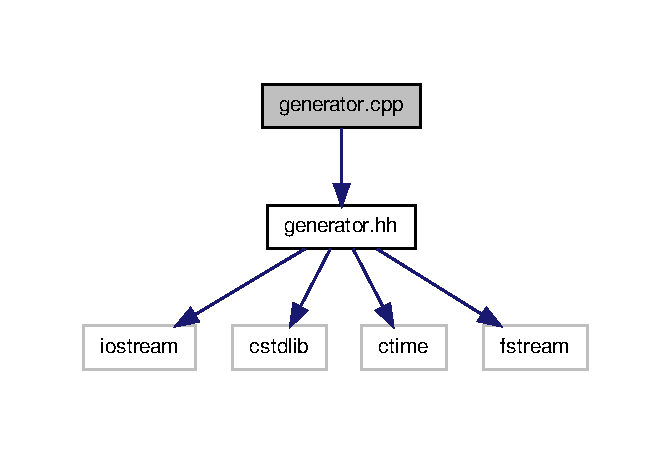
\includegraphics[width=322pt]{generator_8cpp__incl}
\end{center}
\end{figure}
\subsection*{\-Funkcje}
\begin{DoxyCompactItemize}
\item 
void \hyperlink{generator_8cpp_a8a338f908bb9996d5b01aab4439e8a56}{generuj} (char $\ast$nazwa, int rozmiar)
\begin{DoxyCompactList}\small\item\em generuje plik $\ast$.txt o zadanej ilosci danych i nazwie \end{DoxyCompactList}\end{DoxyCompactItemize}


\subsection{\-Dokumentacja funkcji}
\hypertarget{generator_8cpp_a8a338f908bb9996d5b01aab4439e8a56}{\index{generator.\-cpp@{generator.\-cpp}!generuj@{generuj}}
\index{generuj@{generuj}!generator.cpp@{generator.\-cpp}}
\subsubsection[{generuj}]{\setlength{\rightskip}{0pt plus 5cm}void {\bf generuj} (
\begin{DoxyParamCaption}
\item[{char $\ast$}]{nazwa, }
\item[{int}]{rozmiar}
\end{DoxyParamCaption}
)}}\label{generator_8cpp_a8a338f908bb9996d5b01aab4439e8a56}


generuje plik $\ast$.txt o zadanej ilosci danych i nazwie 

\-W pliku umieszczane sa liczby naturalne od 1 wzwyrz w pierwszym wierszu umieszczana jest liczba mowiaca o ilosci wierszy danych. 
\begin{DoxyParams}{\-Parametry}
{\em nazwa} & -\/ utworzonego pliku \\
\hline
{\em rozmiar} & -\/ ilosc wierszy sanych \\
\hline
\end{DoxyParams}


\-Definicja w linii 19 pliku generator.\-cpp.



\-Oto graf wywoływań tej funkcji\-:\nopagebreak
\begin{figure}[H]
\begin{center}
\leavevmode
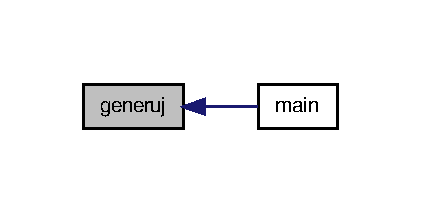
\includegraphics[width=202pt]{generator_8cpp_a8a338f908bb9996d5b01aab4439e8a56_icgraph}
\end{center}
\end{figure}



\hypertarget{generator_8hh}{\section{\-Dokumentacja pliku generator.\-hh}
\label{generator_8hh}\index{generator.\-hh@{generator.\-hh}}
}
{\ttfamily \#include $<$iostream$>$}\*
{\ttfamily \#include $<$cstdlib$>$}\*
{\ttfamily \#include $<$ctime$>$}\*
{\ttfamily \#include $<$fstream$>$}\*
\-Wykres zależności załączania dla generator.\-hh\-:\nopagebreak
\begin{figure}[H]
\begin{center}
\leavevmode
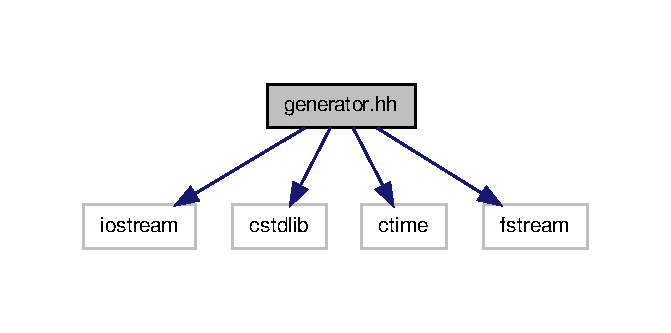
\includegraphics[width=322pt]{generator_8hh__incl}
\end{center}
\end{figure}
\-Ten wykres pokazuje, które pliki bezpośrednio lub pośrednio załączają ten plik\-:\nopagebreak
\begin{figure}[H]
\begin{center}
\leavevmode
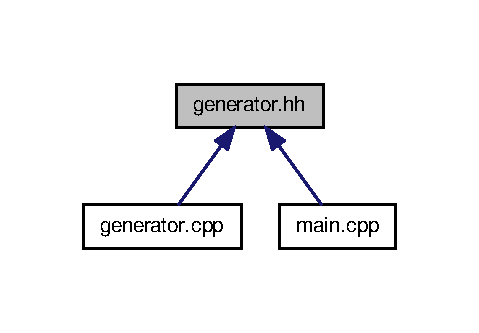
\includegraphics[width=230pt]{generator_8hh__dep__incl}
\end{center}
\end{figure}
\subsection*{\-Funkcje}
\begin{DoxyCompactItemize}
\item 
void \hyperlink{generator_8hh_a8a338f908bb9996d5b01aab4439e8a56}{generuj} (char $\ast$nazwa, int rozmiar)
\begin{DoxyCompactList}\small\item\em generuje plik $\ast$.txt o zadanej ilosci danych i nazwie \end{DoxyCompactList}\end{DoxyCompactItemize}


\subsection{\-Dokumentacja funkcji}
\hypertarget{generator_8hh_a8a338f908bb9996d5b01aab4439e8a56}{\index{generator.\-hh@{generator.\-hh}!generuj@{generuj}}
\index{generuj@{generuj}!generator.hh@{generator.\-hh}}
\subsubsection[{generuj}]{\setlength{\rightskip}{0pt plus 5cm}void {\bf generuj} (
\begin{DoxyParamCaption}
\item[{char $\ast$}]{nazwa, }
\item[{int}]{rozmiar}
\end{DoxyParamCaption}
)}}\label{generator_8hh_a8a338f908bb9996d5b01aab4439e8a56}


generuje plik $\ast$.txt o zadanej ilosci danych i nazwie 

\-W pliku umieszczane sa liczby naturalne od 1 wzwyrz w pierwszym wierszu umieszczana jest liczba mowiaca o ilosci wierszy danych. 
\begin{DoxyParams}{\-Parametry}
{\em nazwa} & -\/ utworzonego pliku \\
\hline
{\em rozmiar} & -\/ ilosc wierszy sanych \\
\hline
\end{DoxyParams}


\-Definicja w linii 19 pliku generator.\-cpp.



\-Oto graf wywoływań tej funkcji\-:\nopagebreak
\begin{figure}[H]
\begin{center}
\leavevmode
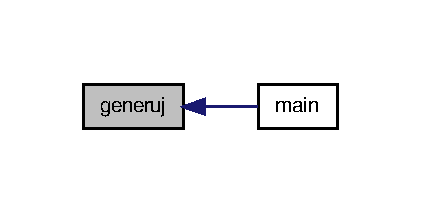
\includegraphics[width=202pt]{generator_8hh_a8a338f908bb9996d5b01aab4439e8a56_icgraph}
\end{center}
\end{figure}



\hypertarget{heap_8cpp}{\section{\-Dokumentacja pliku heap.\-cpp}
\label{heap_8cpp}\index{heap.\-cpp@{heap.\-cpp}}
}
{\ttfamily \#include \char`\"{}heap.\-hh\char`\"{}}\*
\-Wykres zależności załączania dla heap.\-cpp\-:\nopagebreak
\begin{figure}[H]
\begin{center}
\leavevmode
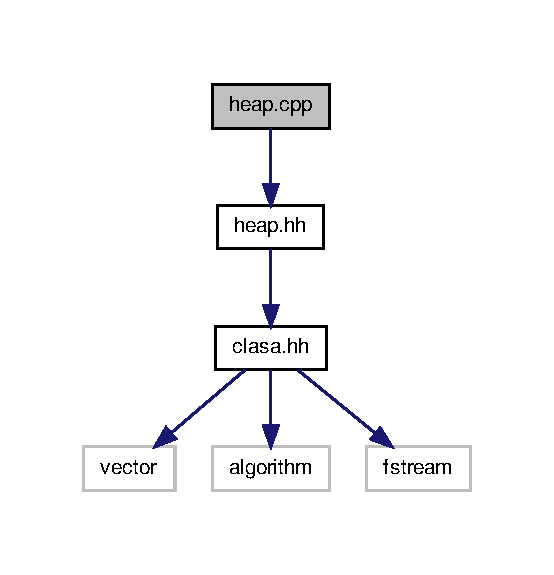
\includegraphics[width=266pt]{heap_8cpp__incl}
\end{center}
\end{figure}
\subsection*{\-Funkcje}
\begin{DoxyCompactItemize}
\item 
void \hyperlink{heap_8cpp_aaa3956ba23a7ef4819511e8f9726bbb9}{sasiedzi} (int pozycja, int $\ast$wyzej, int $\ast$lewy, int $\ast$prawy)
\begin{DoxyCompactList}\small\item\em funkcja oblicza indeksy galezi wezla. \end{DoxyCompactList}\item 
void \hyperlink{heap_8cpp_a57ca91ed761880e713ce3321d51b9ca3}{heap} (\hyperlink{classdane}{dane} \&zbior, int rozmiar)
\begin{DoxyCompactList}\small\item\em porzadkuje kopiec \end{DoxyCompactList}\item 
void \hyperlink{heap_8cpp_af0e033b3011366bedae3722020bac21a}{wez} (\hyperlink{classdane}{dane} \&zbior, int \&rozmiar)
\begin{DoxyCompactList}\small\item\em przeklada najstarszy wezel (najwieksza wartosc) na koniec wektora \end{DoxyCompactList}\item 
void \hyperlink{heap_8cpp_aa5d4073154327bd623b36d1070aa2827}{heap\-\_\-sort} (\hyperlink{classdane}{dane} \&zbior)
\begin{DoxyCompactList}\small\item\em wywoluje w petli funkcje budujaca kopiec oraz sciagajaca najwieksza wartosc \end{DoxyCompactList}\end{DoxyCompactItemize}


\subsection{\-Dokumentacja funkcji}
\hypertarget{heap_8cpp_a57ca91ed761880e713ce3321d51b9ca3}{\index{heap.\-cpp@{heap.\-cpp}!heap@{heap}}
\index{heap@{heap}!heap.cpp@{heap.\-cpp}}
\subsubsection[{heap}]{\setlength{\rightskip}{0pt plus 5cm}void {\bf heap} (
\begin{DoxyParamCaption}
\item[{{\bf dane} \&}]{zbior, }
\item[{int}]{rozmiar}
\end{DoxyParamCaption}
)}}\label{heap_8cpp_a57ca91ed761880e713ce3321d51b9ca3}


porzadkuje kopiec 

funkcja przeglada kopiec od dolnego rzedu wezlow w gore. \-Po przez operacje porownania wypycha wieksze elemnty w gore kopca. 
\begin{DoxyParams}{\-Parametry}
{\em zbior} & zbior elementow do posortowania \\
\hline
{\em rozmiar} & rozmiar problemu \\
\hline
\end{DoxyParams}
przegladamy wezly a nie liscie

wezly sa indekowane od 1 

\-Definicja w linii 32 pliku heap.\-cpp.



\-Oto graf wywołań dla tej funkcji\-:\nopagebreak
\begin{figure}[H]
\begin{center}
\leavevmode
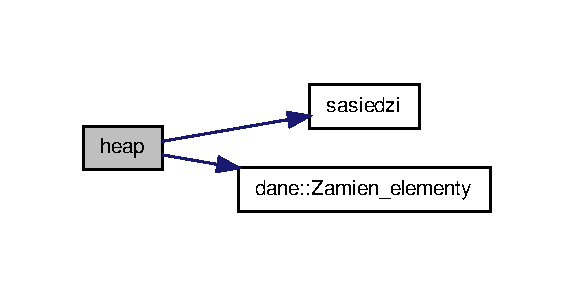
\includegraphics[width=276pt]{heap_8cpp_a57ca91ed761880e713ce3321d51b9ca3_cgraph}
\end{center}
\end{figure}




\-Oto graf wywoływań tej funkcji\-:\nopagebreak
\begin{figure}[H]
\begin{center}
\leavevmode
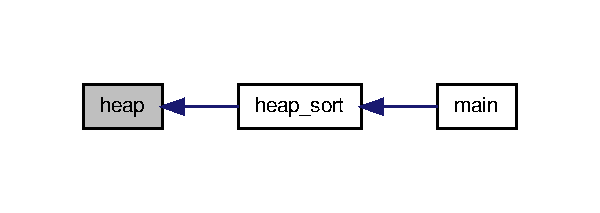
\includegraphics[width=288pt]{heap_8cpp_a57ca91ed761880e713ce3321d51b9ca3_icgraph}
\end{center}
\end{figure}


\hypertarget{heap_8cpp_aa5d4073154327bd623b36d1070aa2827}{\index{heap.\-cpp@{heap.\-cpp}!heap\-\_\-sort@{heap\-\_\-sort}}
\index{heap\-\_\-sort@{heap\-\_\-sort}!heap.cpp@{heap.\-cpp}}
\subsubsection[{heap\-\_\-sort}]{\setlength{\rightskip}{0pt plus 5cm}void {\bf heap\-\_\-sort} (
\begin{DoxyParamCaption}
\item[{{\bf dane} \&}]{zbior}
\end{DoxyParamCaption}
)}}\label{heap_8cpp_aa5d4073154327bd623b36d1070aa2827}


wywoluje w petli funkcje budujaca kopiec oraz sciagajaca najwieksza wartosc 


\begin{DoxyParams}{\-Parametry}
{\em zbior} & \\
\hline
\end{DoxyParams}


\-Definicja w linii 62 pliku heap.\-cpp.



\-Oto graf wywołań dla tej funkcji\-:\nopagebreak
\begin{figure}[H]
\begin{center}
\leavevmode
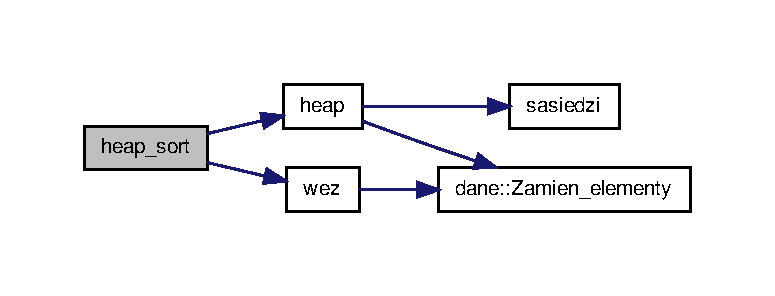
\includegraphics[width=350pt]{heap_8cpp_aa5d4073154327bd623b36d1070aa2827_cgraph}
\end{center}
\end{figure}




\-Oto graf wywoływań tej funkcji\-:\nopagebreak
\begin{figure}[H]
\begin{center}
\leavevmode
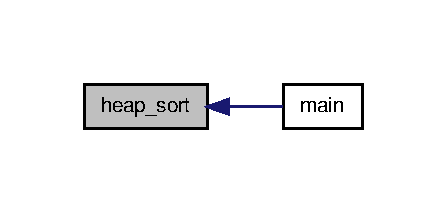
\includegraphics[width=214pt]{heap_8cpp_aa5d4073154327bd623b36d1070aa2827_icgraph}
\end{center}
\end{figure}


\hypertarget{heap_8cpp_aaa3956ba23a7ef4819511e8f9726bbb9}{\index{heap.\-cpp@{heap.\-cpp}!sasiedzi@{sasiedzi}}
\index{sasiedzi@{sasiedzi}!heap.cpp@{heap.\-cpp}}
\subsubsection[{sasiedzi}]{\setlength{\rightskip}{0pt plus 5cm}void {\bf sasiedzi} (
\begin{DoxyParamCaption}
\item[{int}]{pozycja, }
\item[{int $\ast$}]{wyzej, }
\item[{int $\ast$}]{lewy, }
\item[{int $\ast$}]{prawy}
\end{DoxyParamCaption}
)}}\label{heap_8cpp_aaa3956ba23a7ef4819511e8f9726bbb9}


funkcja oblicza indeksy galezi wezla. 

wezly sa indeksowane od 1 wiec w oniesieniu do wektora trzeba odjac 1. 
\begin{DoxyParams}{\-Parametry}
{\em pozycja} & bierzacy wezele \\
\hline
{\em wyzej} & wezel mlodszy \\
\hline
{\em lewy} & wezel starszy \\
\hline
{\em prawy} & wezel starszy \\
\hline
\end{DoxyParams}


\-Definicja w linii 19 pliku heap.\-cpp.



\-Oto graf wywoływań tej funkcji\-:\nopagebreak
\begin{figure}[H]
\begin{center}
\leavevmode
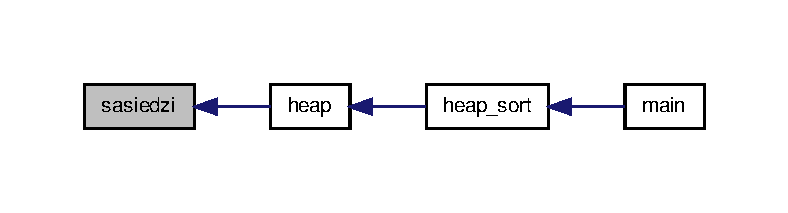
\includegraphics[width=350pt]{heap_8cpp_aaa3956ba23a7ef4819511e8f9726bbb9_icgraph}
\end{center}
\end{figure}


\hypertarget{heap_8cpp_af0e033b3011366bedae3722020bac21a}{\index{heap.\-cpp@{heap.\-cpp}!wez@{wez}}
\index{wez@{wez}!heap.cpp@{heap.\-cpp}}
\subsubsection[{wez}]{\setlength{\rightskip}{0pt plus 5cm}void {\bf wez} (
\begin{DoxyParamCaption}
\item[{{\bf dane} \&}]{zbior, }
\item[{int \&}]{rozmiar}
\end{DoxyParamCaption}
)}}\label{heap_8cpp_af0e033b3011366bedae3722020bac21a}


przeklada najstarszy wezel (najwieksza wartosc) na koniec wektora 


\begin{DoxyParams}{\-Parametry}
{\em zbior} & dane do upozadkowania \\
\hline
{\em rozmiar} & problemu \\
\hline
\end{DoxyParams}
znowu te indeksy 

\-Definicja w linii 52 pliku heap.\-cpp.



\-Oto graf wywołań dla tej funkcji\-:\nopagebreak
\begin{figure}[H]
\begin{center}
\leavevmode
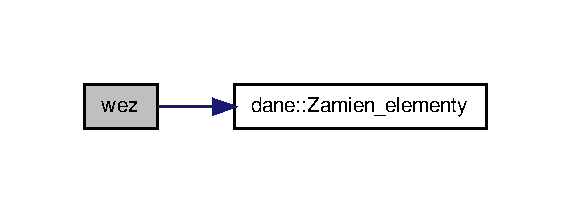
\includegraphics[width=274pt]{heap_8cpp_af0e033b3011366bedae3722020bac21a_cgraph}
\end{center}
\end{figure}




\-Oto graf wywoływań tej funkcji\-:\nopagebreak
\begin{figure}[H]
\begin{center}
\leavevmode
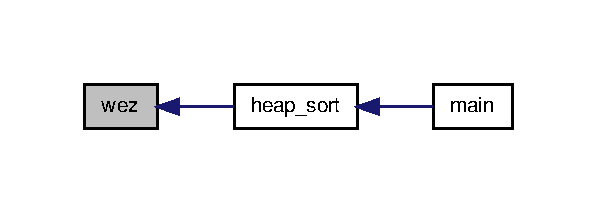
\includegraphics[width=286pt]{heap_8cpp_af0e033b3011366bedae3722020bac21a_icgraph}
\end{center}
\end{figure}



\hypertarget{heap_8hh}{\section{\-Dokumentacja pliku heap.\-hh}
\label{heap_8hh}\index{heap.\-hh@{heap.\-hh}}
}
{\ttfamily \#include \char`\"{}clasa.\-hh\char`\"{}}\*
\-Wykres zależności załączania dla heap.\-hh\-:\nopagebreak
\begin{figure}[H]
\begin{center}
\leavevmode
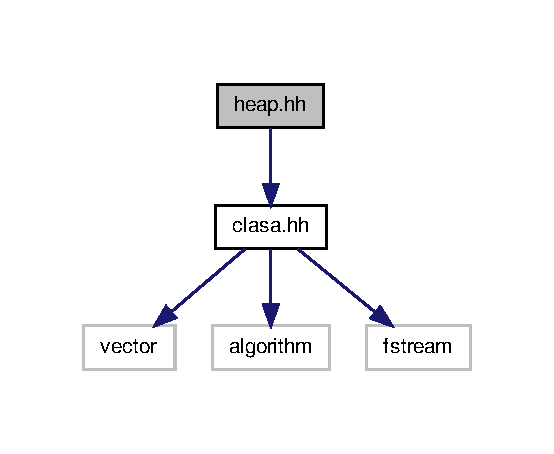
\includegraphics[width=266pt]{heap_8hh__incl}
\end{center}
\end{figure}
\-Ten wykres pokazuje, które pliki bezpośrednio lub pośrednio załączają ten plik\-:\nopagebreak
\begin{figure}[H]
\begin{center}
\leavevmode
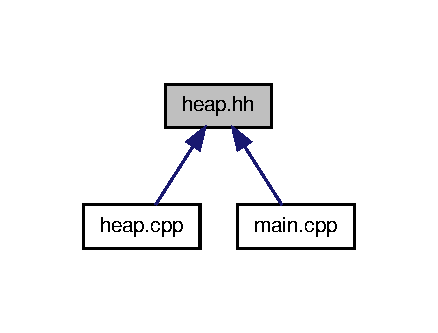
\includegraphics[width=210pt]{heap_8hh__dep__incl}
\end{center}
\end{figure}
\subsection*{\-Funkcje}
\begin{DoxyCompactItemize}
\item 
void \hyperlink{heap_8hh_aa5d4073154327bd623b36d1070aa2827}{heap\-\_\-sort} (\hyperlink{classdane}{dane} \&zbior)
\begin{DoxyCompactList}\small\item\em wywoluje w petli funkcje budujaca kopiec oraz sciagajaca najwieksza wartosc \end{DoxyCompactList}\end{DoxyCompactItemize}


\subsection{\-Dokumentacja funkcji}
\hypertarget{heap_8hh_aa5d4073154327bd623b36d1070aa2827}{\index{heap.\-hh@{heap.\-hh}!heap\-\_\-sort@{heap\-\_\-sort}}
\index{heap\-\_\-sort@{heap\-\_\-sort}!heap.hh@{heap.\-hh}}
\subsubsection[{heap\-\_\-sort}]{\setlength{\rightskip}{0pt plus 5cm}void {\bf heap\-\_\-sort} (
\begin{DoxyParamCaption}
\item[{{\bf dane} \&}]{zbior}
\end{DoxyParamCaption}
)}}\label{heap_8hh_aa5d4073154327bd623b36d1070aa2827}


wywoluje w petli funkcje budujaca kopiec oraz sciagajaca najwieksza wartosc 


\begin{DoxyParams}{\-Parametry}
{\em zbior} & \\
\hline
\end{DoxyParams}


\-Definicja w linii 62 pliku heap.\-cpp.



\-Oto graf wywołań dla tej funkcji\-:\nopagebreak
\begin{figure}[H]
\begin{center}
\leavevmode
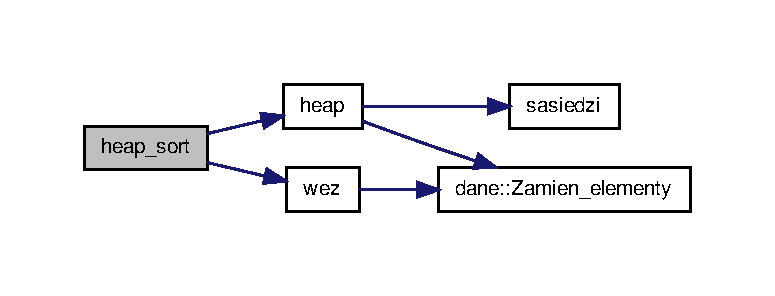
\includegraphics[width=350pt]{heap_8hh_aa5d4073154327bd623b36d1070aa2827_cgraph}
\end{center}
\end{figure}




\-Oto graf wywoływań tej funkcji\-:\nopagebreak
\begin{figure}[H]
\begin{center}
\leavevmode
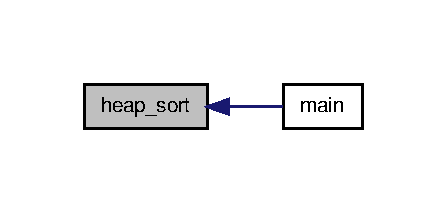
\includegraphics[width=214pt]{heap_8hh_aa5d4073154327bd623b36d1070aa2827_icgraph}
\end{center}
\end{figure}



\hypertarget{main_8cpp}{\section{\-Dokumentacja pliku main.\-cpp}
\label{main_8cpp}\index{main.\-cpp@{main.\-cpp}}
}
{\ttfamily \#include $<$iostream$>$}\*
{\ttfamily \#include \char`\"{}funkcje.\-hh\char`\"{}}\*
{\ttfamily \#include \char`\"{}clasa.\-hh\char`\"{}}\*
{\ttfamily \#include $<$fstream$>$}\*
{\ttfamily \#include $<$vector$>$}\*
{\ttfamily \#include \char`\"{}generator.\-hh\char`\"{}}\*
{\ttfamily \#include \char`\"{}quick.\-hh\char`\"{}}\*
{\ttfamily \#include \char`\"{}merge.\-hh\char`\"{}}\*
{\ttfamily \#include \char`\"{}heap.\-hh\char`\"{}}\*
{\ttfamily \#include \char`\"{}stoper.\-hh\char`\"{}}\*
\-Wykres zależności załączania dla main.\-cpp\-:\nopagebreak
\begin{figure}[H]
\begin{center}
\leavevmode
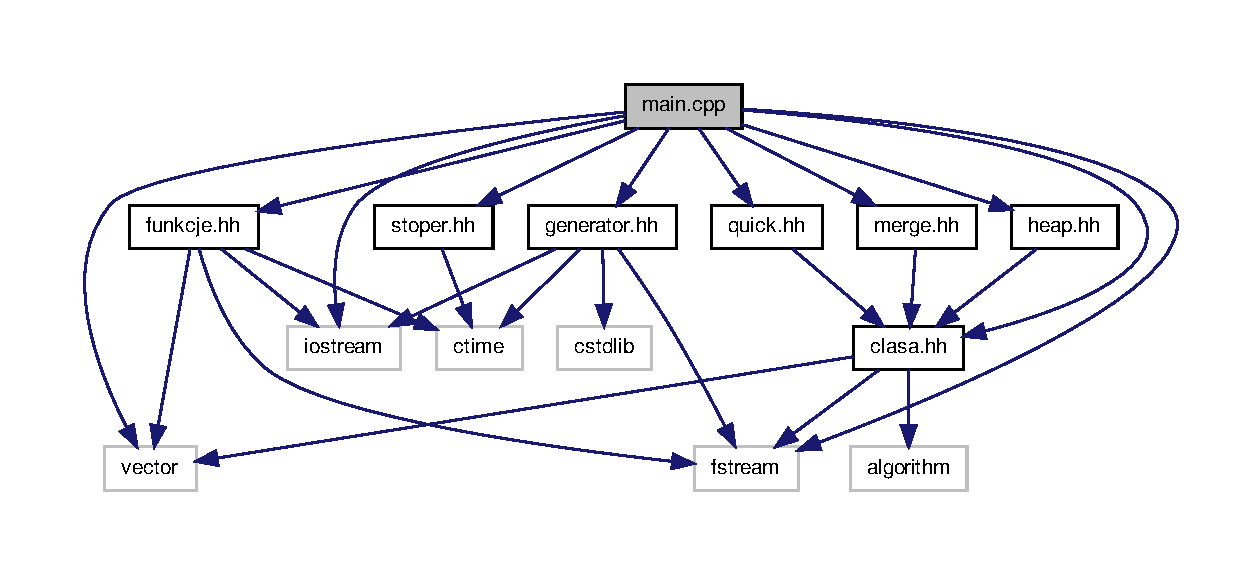
\includegraphics[width=350pt]{main_8cpp__incl}
\end{center}
\end{figure}
\subsection*{\-Definicje}
\begin{DoxyCompactItemize}
\item 
\#define \hyperlink{main_8cpp_a5b91f08c2050b0e3b6b88de7a09bb6f8}{\-S\-R\-E\-D\-N\-I\-A\-\_\-\-Z}~5
\end{DoxyCompactItemize}
\subsection*{\-Funkcje}
\begin{DoxyCompactItemize}
\item 
int \hyperlink{main_8cpp_ae66f6b31b5ad750f1fe042a706a4e3d4}{main} ()
\end{DoxyCompactItemize}
\subsection*{\-Zmienne}
\begin{DoxyCompactItemize}
\item 
fstream \hyperlink{main_8cpp_a689b27a44e1598a3ce71d53c8000f64a}{in}
\item 
fstream \hyperlink{main_8cpp_a67ff2f1724c27ce37872c5d75172f4ff}{wynik}
\end{DoxyCompactItemize}


\subsection{\-Dokumentacja definicji}
\hypertarget{main_8cpp_a5b91f08c2050b0e3b6b88de7a09bb6f8}{\index{main.\-cpp@{main.\-cpp}!\-S\-R\-E\-D\-N\-I\-A\-\_\-\-Z@{\-S\-R\-E\-D\-N\-I\-A\-\_\-\-Z}}
\index{\-S\-R\-E\-D\-N\-I\-A\-\_\-\-Z@{\-S\-R\-E\-D\-N\-I\-A\-\_\-\-Z}!main.cpp@{main.\-cpp}}
\subsubsection[{\-S\-R\-E\-D\-N\-I\-A\-\_\-\-Z}]{\setlength{\rightskip}{0pt plus 5cm}\#define {\bf \-S\-R\-E\-D\-N\-I\-A\-\_\-\-Z}~5}}\label{main_8cpp_a5b91f08c2050b0e3b6b88de7a09bb6f8}


\-Definicja w linii 9 pliku main.\-cpp.



\subsection{\-Dokumentacja funkcji}
\hypertarget{main_8cpp_ae66f6b31b5ad750f1fe042a706a4e3d4}{\index{main.\-cpp@{main.\-cpp}!main@{main}}
\index{main@{main}!main.cpp@{main.\-cpp}}
\subsubsection[{main}]{\setlength{\rightskip}{0pt plus 5cm}int {\bf main} (
\begin{DoxyParamCaption}
{}
\end{DoxyParamCaption}
)}}\label{main_8cpp_ae66f6b31b5ad750f1fe042a706a4e3d4}


\-Definicja w linii 27 pliku main.\-cpp.



\-Oto graf wywołań dla tej funkcji\-:\nopagebreak
\begin{figure}[H]
\begin{center}
\leavevmode
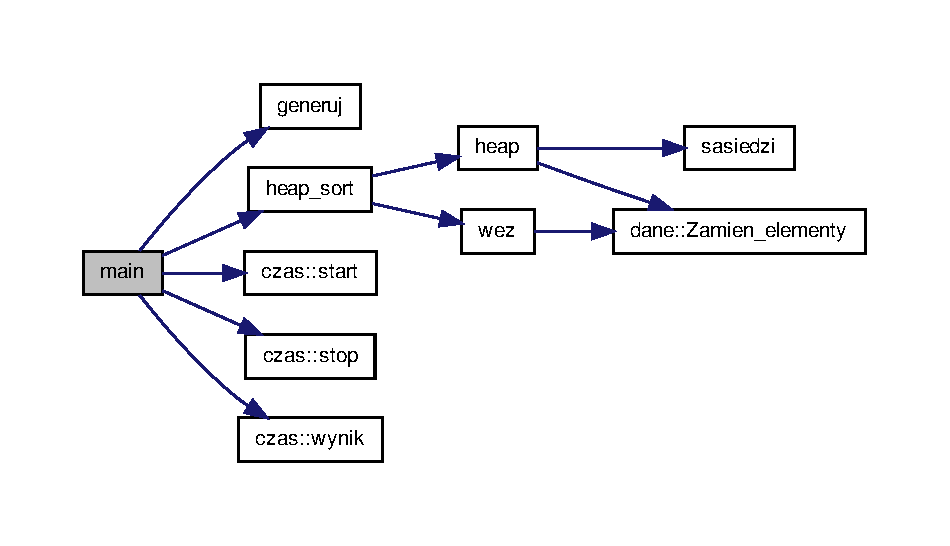
\includegraphics[width=350pt]{main_8cpp_ae66f6b31b5ad750f1fe042a706a4e3d4_cgraph}
\end{center}
\end{figure}




\subsection{\-Dokumentacja zmiennych}
\hypertarget{main_8cpp_a689b27a44e1598a3ce71d53c8000f64a}{\index{main.\-cpp@{main.\-cpp}!in@{in}}
\index{in@{in}!main.cpp@{main.\-cpp}}
\subsubsection[{in}]{\setlength{\rightskip}{0pt plus 5cm}fstream {\bf in}}}\label{main_8cpp_a689b27a44e1598a3ce71d53c8000f64a}


\-Definicja w linii 24 pliku main.\-cpp.

\hypertarget{main_8cpp_a67ff2f1724c27ce37872c5d75172f4ff}{\index{main.\-cpp@{main.\-cpp}!wynik@{wynik}}
\index{wynik@{wynik}!main.cpp@{main.\-cpp}}
\subsubsection[{wynik}]{\setlength{\rightskip}{0pt plus 5cm}fstream {\bf wynik}}}\label{main_8cpp_a67ff2f1724c27ce37872c5d75172f4ff}


\-Definicja w linii 25 pliku main.\-cpp.


\hypertarget{merge_8cpp}{\section{\-Dokumentacja pliku merge.\-cpp}
\label{merge_8cpp}\index{merge.\-cpp@{merge.\-cpp}}
}
{\ttfamily \#include \char`\"{}merge.\-hh\char`\"{}}\*
\-Wykres zależności załączania dla merge.\-cpp\-:\nopagebreak
\begin{figure}[H]
\begin{center}
\leavevmode
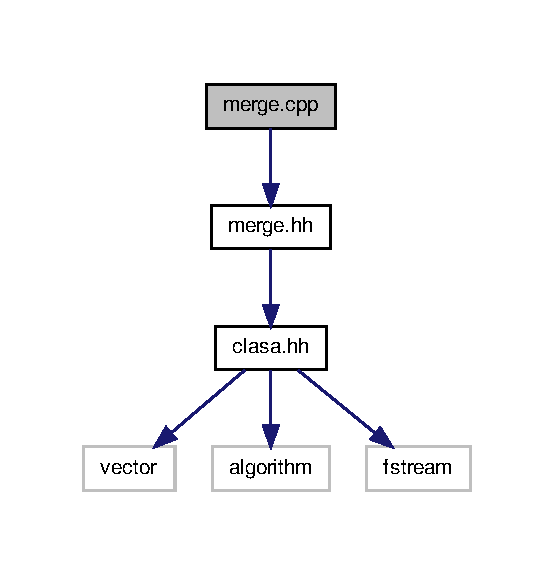
\includegraphics[width=266pt]{merge_8cpp__incl}
\end{center}
\end{figure}
\subsection*{\-Funkcje}
\begin{DoxyCompactItemize}
\item 
void \hyperlink{merge_8cpp_a80562ba6e89a73c71c9c2ec3b3220355}{merge} (\hyperlink{classdane}{dane} \&zbior, int poczatek, int srodek, int koniec)
\begin{DoxyCompactList}\small\item\em scala zbiory sortujac je \end{DoxyCompactList}\item 
void \hyperlink{merge_8cpp_a21cc64084ad14436ca30fc77c41765d3}{merge\-\_\-sort} (\hyperlink{classdane}{dane} \&zbior, int poczatek, int koniec)
\begin{DoxyCompactList}\small\item\em dzieli wektor na mniejsze czesci \end{DoxyCompactList}\end{DoxyCompactItemize}


\subsection{\-Dokumentacja funkcji}
\hypertarget{merge_8cpp_a80562ba6e89a73c71c9c2ec3b3220355}{\index{merge.\-cpp@{merge.\-cpp}!merge@{merge}}
\index{merge@{merge}!merge.cpp@{merge.\-cpp}}
\subsubsection[{merge}]{\setlength{\rightskip}{0pt plus 5cm}void {\bf merge} (
\begin{DoxyParamCaption}
\item[{{\bf dane} \&}]{zbior, }
\item[{int}]{poczatek, }
\item[{int}]{srodek, }
\item[{int}]{koniec}
\end{DoxyParamCaption}
)}}\label{merge_8cpp_a80562ba6e89a73c71c9c2ec3b3220355}


scala zbiory sortujac je 


\begin{DoxyParams}{\-Parametry}
{\em zbior} & dane wejsciowe \\
\hline
{\em poczatek} & wskaznik na poczatek zbioru \\
\hline
{\em srodek} & wskaznik na srodek zbioru \\
\hline
{\em koniec} & wskaznik na koniec zbioru \\
\hline
\end{DoxyParams}


\-Definicja w linii 17 pliku merge.\-cpp.



\-Oto graf wywoływań tej funkcji\-:\nopagebreak
\begin{figure}[H]
\begin{center}
\leavevmode
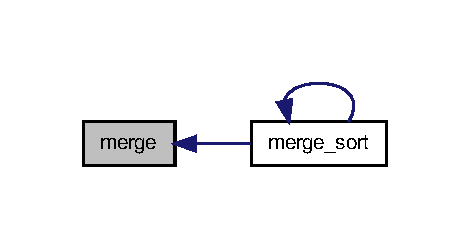
\includegraphics[width=226pt]{merge_8cpp_a80562ba6e89a73c71c9c2ec3b3220355_icgraph}
\end{center}
\end{figure}


\hypertarget{merge_8cpp_a21cc64084ad14436ca30fc77c41765d3}{\index{merge.\-cpp@{merge.\-cpp}!merge\-\_\-sort@{merge\-\_\-sort}}
\index{merge\-\_\-sort@{merge\-\_\-sort}!merge.cpp@{merge.\-cpp}}
\subsubsection[{merge\-\_\-sort}]{\setlength{\rightskip}{0pt plus 5cm}void {\bf merge\-\_\-sort} (
\begin{DoxyParamCaption}
\item[{{\bf dane} \&}]{zbior, }
\item[{int}]{poczatek, }
\item[{int}]{koniec}
\end{DoxyParamCaption}
)}}\label{merge_8cpp_a21cc64084ad14436ca30fc77c41765d3}


dzieli wektor na mniejsze czesci 

poprzez rekurencyjne wywolywanie funkcji 'dzieli' vector na jednoelementowe czesci. \-Nastepnie poprzez wywyolanie funkcji \hyperlink{merge_8cpp_a80562ba6e89a73c71c9c2ec3b3220355}{merge()} scala i sortuje je. 
\begin{DoxyParams}{\-Parametry}
{\em zbior} & \\
\hline
{\em poczatek} & \\
\hline
{\em koniec} & \\
\hline
\end{DoxyParams}


\-Definicja w linii 59 pliku merge.\-cpp.



\-Oto graf wywołań dla tej funkcji\-:\nopagebreak
\begin{figure}[H]
\begin{center}
\leavevmode
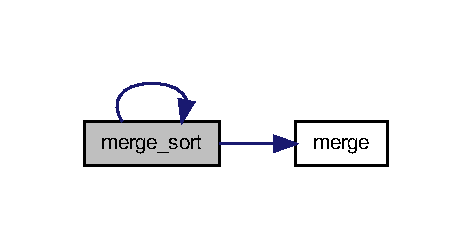
\includegraphics[width=226pt]{merge_8cpp_a21cc64084ad14436ca30fc77c41765d3_cgraph}
\end{center}
\end{figure}




\-Oto graf wywoływań tej funkcji\-:\nopagebreak
\begin{figure}[H]
\begin{center}
\leavevmode
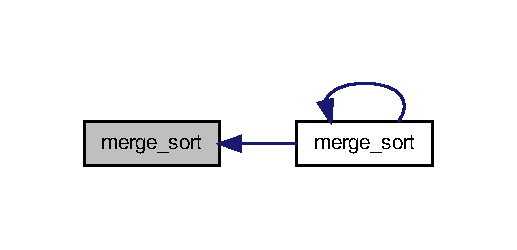
\includegraphics[width=248pt]{merge_8cpp_a21cc64084ad14436ca30fc77c41765d3_icgraph}
\end{center}
\end{figure}



\hypertarget{merge_8hh}{\section{\-Dokumentacja pliku merge.\-hh}
\label{merge_8hh}\index{merge.\-hh@{merge.\-hh}}
}
{\ttfamily \#include \char`\"{}clasa.\-hh\char`\"{}}\*
\-Wykres zależności załączania dla merge.\-hh\-:\nopagebreak
\begin{figure}[H]
\begin{center}
\leavevmode
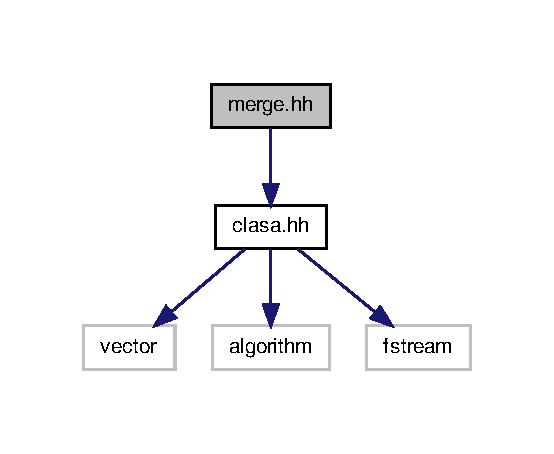
\includegraphics[width=266pt]{merge_8hh__incl}
\end{center}
\end{figure}
\-Ten wykres pokazuje, które pliki bezpośrednio lub pośrednio załączają ten plik\-:\nopagebreak
\begin{figure}[H]
\begin{center}
\leavevmode
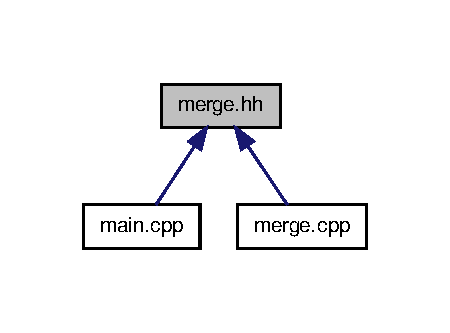
\includegraphics[width=216pt]{merge_8hh__dep__incl}
\end{center}
\end{figure}
\subsection*{\-Funkcje}
\begin{DoxyCompactItemize}
\item 
void \hyperlink{merge_8hh_a80562ba6e89a73c71c9c2ec3b3220355}{merge} (\hyperlink{classdane}{dane} \&zbior, int poczatek, int srodek, int koniec)
\begin{DoxyCompactList}\small\item\em scala zbiory sortujac je \end{DoxyCompactList}\item 
void \hyperlink{merge_8hh_a21cc64084ad14436ca30fc77c41765d3}{merge\-\_\-sort} (\hyperlink{classdane}{dane} \&zbior, int poczatek, int koniec)
\begin{DoxyCompactList}\small\item\em dzieli wektor na mniejsze czesci \end{DoxyCompactList}\end{DoxyCompactItemize}


\subsection{\-Dokumentacja funkcji}
\hypertarget{merge_8hh_a80562ba6e89a73c71c9c2ec3b3220355}{\index{merge.\-hh@{merge.\-hh}!merge@{merge}}
\index{merge@{merge}!merge.hh@{merge.\-hh}}
\subsubsection[{merge}]{\setlength{\rightskip}{0pt plus 5cm}void {\bf merge} (
\begin{DoxyParamCaption}
\item[{{\bf dane} \&}]{zbior, }
\item[{int}]{poczatek, }
\item[{int}]{srodek, }
\item[{int}]{koniec}
\end{DoxyParamCaption}
)}}\label{merge_8hh_a80562ba6e89a73c71c9c2ec3b3220355}


scala zbiory sortujac je 


\begin{DoxyParams}{\-Parametry}
{\em zbior} & dane wejsciowe \\
\hline
{\em poczatek} & wskaznik na poczatek zbioru \\
\hline
{\em srodek} & wskaznik na srodek zbioru \\
\hline
{\em koniec} & wskaznik na koniec zbioru \\
\hline
\end{DoxyParams}


\-Definicja w linii 17 pliku merge.\-cpp.



\-Oto graf wywoływań tej funkcji\-:\nopagebreak
\begin{figure}[H]
\begin{center}
\leavevmode
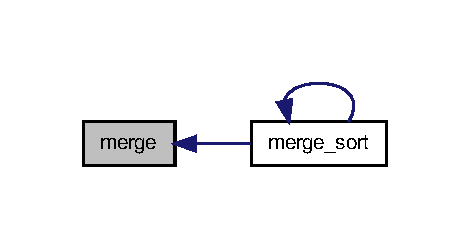
\includegraphics[width=226pt]{merge_8hh_a80562ba6e89a73c71c9c2ec3b3220355_icgraph}
\end{center}
\end{figure}


\hypertarget{merge_8hh_a21cc64084ad14436ca30fc77c41765d3}{\index{merge.\-hh@{merge.\-hh}!merge\-\_\-sort@{merge\-\_\-sort}}
\index{merge\-\_\-sort@{merge\-\_\-sort}!merge.hh@{merge.\-hh}}
\subsubsection[{merge\-\_\-sort}]{\setlength{\rightskip}{0pt plus 5cm}void {\bf merge\-\_\-sort} (
\begin{DoxyParamCaption}
\item[{{\bf dane} \&}]{zbior, }
\item[{int}]{poczatek, }
\item[{int}]{koniec}
\end{DoxyParamCaption}
)}}\label{merge_8hh_a21cc64084ad14436ca30fc77c41765d3}


dzieli wektor na mniejsze czesci 

poprzez rekurencyjne wywolywanie funkcji 'dzieli' vector na jednoelementowe czesci. \-Nastepnie poprzez wywyolanie funkcji \hyperlink{merge_8cpp_a80562ba6e89a73c71c9c2ec3b3220355}{merge()} scala i sortuje je. 
\begin{DoxyParams}{\-Parametry}
{\em zbior} & \\
\hline
{\em poczatek} & \\
\hline
{\em koniec} & \\
\hline
\end{DoxyParams}


\-Definicja w linii 59 pliku merge.\-cpp.



\-Oto graf wywołań dla tej funkcji\-:\nopagebreak
\begin{figure}[H]
\begin{center}
\leavevmode
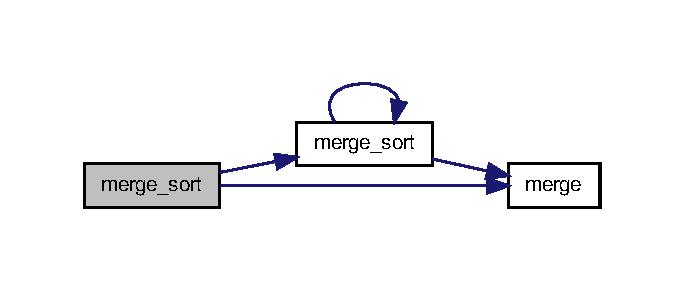
\includegraphics[width=328pt]{merge_8hh_a21cc64084ad14436ca30fc77c41765d3_cgraph}
\end{center}
\end{figure}




\-Oto graf wywoływań tej funkcji\-:\nopagebreak
\begin{figure}[H]
\begin{center}
\leavevmode
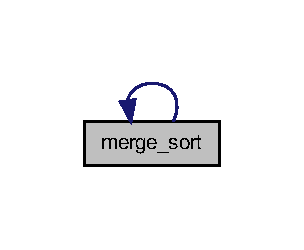
\includegraphics[width=146pt]{merge_8hh_a21cc64084ad14436ca30fc77c41765d3_icgraph}
\end{center}
\end{figure}



\hypertarget{quick_8cpp}{\section{\-Dokumentacja pliku quick.\-cpp}
\label{quick_8cpp}\index{quick.\-cpp@{quick.\-cpp}}
}
{\ttfamily \#include \char`\"{}quick.\-hh\char`\"{}}\*
\-Wykres zależności załączania dla quick.\-cpp\-:\nopagebreak
\begin{figure}[H]
\begin{center}
\leavevmode
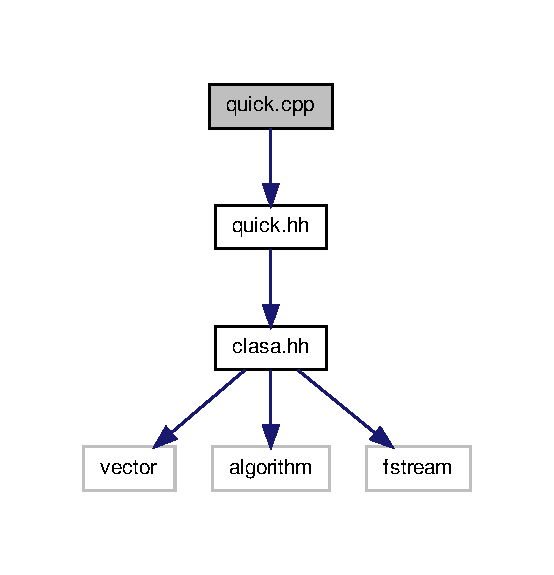
\includegraphics[width=266pt]{quick_8cpp__incl}
\end{center}
\end{figure}
\subsection*{\-Funkcje}
\begin{DoxyCompactItemize}
\item 
void \hyperlink{quick_8cpp_a017b6de88403ed8f5d857c77e57c69d5}{quick} (\hyperlink{classdane}{dane} \&plik, int lewy, int prawy)
\begin{DoxyCompactList}\small\item\em implementacja algorytmu quicksort \end{DoxyCompactList}\end{DoxyCompactItemize}


\subsection{\-Dokumentacja funkcji}
\hypertarget{quick_8cpp_a017b6de88403ed8f5d857c77e57c69d5}{\index{quick.\-cpp@{quick.\-cpp}!quick@{quick}}
\index{quick@{quick}!quick.cpp@{quick.\-cpp}}
\subsubsection[{quick}]{\setlength{\rightskip}{0pt plus 5cm}void {\bf quick} (
\begin{DoxyParamCaption}
\item[{{\bf dane} \&}]{plik, }
\item[{int}]{lewy, }
\item[{int}]{prawy}
\end{DoxyParamCaption}
)}}\label{quick_8cpp_a017b6de88403ed8f5d857c77e57c69d5}


implementacja algorytmu quicksort 


\begin{DoxyParams}{\-Parametry}
{\em plik} & dane do posortowania \\
\hline
{\em lewy} & poczatek ciagu \\
\hline
{\em prawy} & koniec ciagu \\
\hline
\end{DoxyParams}


\-Definicja w linii 22 pliku quick.\-cpp.



\-Oto graf wywołań dla tej funkcji\-:\nopagebreak
\begin{figure}[H]
\begin{center}
\leavevmode
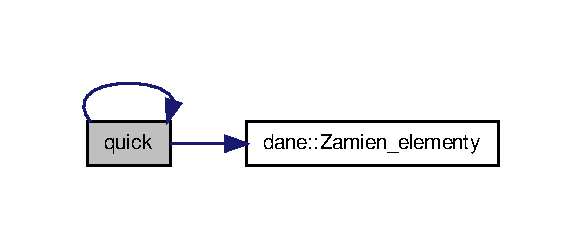
\includegraphics[width=280pt]{quick_8cpp_a017b6de88403ed8f5d857c77e57c69d5_cgraph}
\end{center}
\end{figure}




\-Oto graf wywoływań tej funkcji\-:\nopagebreak
\begin{figure}[H]
\begin{center}
\leavevmode
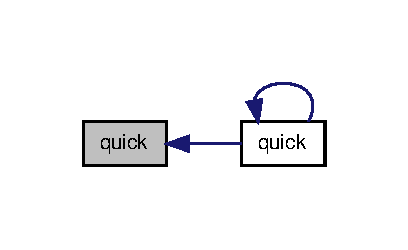
\includegraphics[width=196pt]{quick_8cpp_a017b6de88403ed8f5d857c77e57c69d5_icgraph}
\end{center}
\end{figure}



\hypertarget{quick_8hh}{\section{\-Dokumentacja pliku quick.\-hh}
\label{quick_8hh}\index{quick.\-hh@{quick.\-hh}}
}
{\ttfamily \#include \char`\"{}clasa.\-hh\char`\"{}}\*
\-Wykres zależności załączania dla quick.\-hh\-:\nopagebreak
\begin{figure}[H]
\begin{center}
\leavevmode
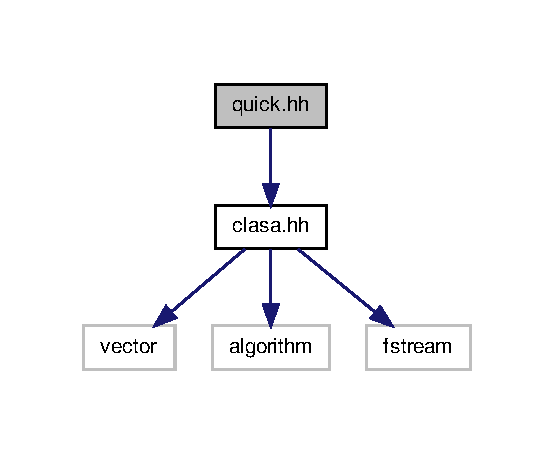
\includegraphics[width=266pt]{quick_8hh__incl}
\end{center}
\end{figure}
\-Ten wykres pokazuje, które pliki bezpośrednio lub pośrednio załączają ten plik\-:\nopagebreak
\begin{figure}[H]
\begin{center}
\leavevmode
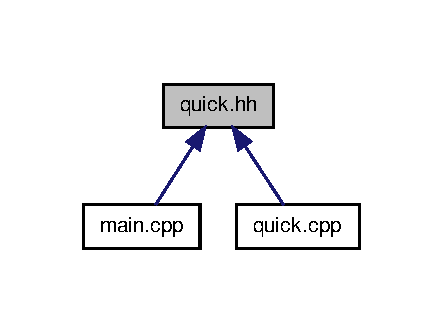
\includegraphics[width=212pt]{quick_8hh__dep__incl}
\end{center}
\end{figure}
\subsection*{\-Funkcje}
\begin{DoxyCompactItemize}
\item 
void \hyperlink{quick_8hh_a017b6de88403ed8f5d857c77e57c69d5}{quick} (\hyperlink{classdane}{dane} \&plik, int lewy, int prawy)
\begin{DoxyCompactList}\small\item\em implementacja algorytmu quicksort \end{DoxyCompactList}\end{DoxyCompactItemize}


\subsection{\-Dokumentacja funkcji}
\hypertarget{quick_8hh_a017b6de88403ed8f5d857c77e57c69d5}{\index{quick.\-hh@{quick.\-hh}!quick@{quick}}
\index{quick@{quick}!quick.hh@{quick.\-hh}}
\subsubsection[{quick}]{\setlength{\rightskip}{0pt plus 5cm}void {\bf quick} (
\begin{DoxyParamCaption}
\item[{{\bf dane} \&}]{plik, }
\item[{int}]{lewy, }
\item[{int}]{prawy}
\end{DoxyParamCaption}
)}}\label{quick_8hh_a017b6de88403ed8f5d857c77e57c69d5}


implementacja algorytmu quicksort 


\begin{DoxyParams}{\-Parametry}
{\em plik} & dane do posortowania \\
\hline
{\em lewy} & poczatek ciagu \\
\hline
{\em prawy} & koniec ciagu \\
\hline
\end{DoxyParams}


\-Definicja w linii 22 pliku quick.\-cpp.



\-Oto graf wywołań dla tej funkcji\-:\nopagebreak
\begin{figure}[H]
\begin{center}
\leavevmode
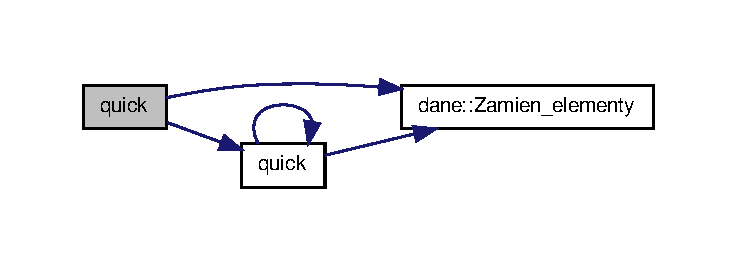
\includegraphics[width=350pt]{quick_8hh_a017b6de88403ed8f5d857c77e57c69d5_cgraph}
\end{center}
\end{figure}




\-Oto graf wywoływań tej funkcji\-:\nopagebreak
\begin{figure}[H]
\begin{center}
\leavevmode
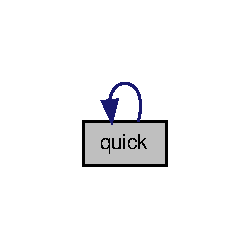
\includegraphics[width=120pt]{quick_8hh_a017b6de88403ed8f5d857c77e57c69d5_icgraph}
\end{center}
\end{figure}



\hypertarget{stoper_8hh}{\section{\-Dokumentacja pliku stoper.\-hh}
\label{stoper_8hh}\index{stoper.\-hh@{stoper.\-hh}}
}
{\ttfamily \#include $<$ctime$>$}\*
\-Wykres zależności załączania dla stoper.\-hh\-:\nopagebreak
\begin{figure}[H]
\begin{center}
\leavevmode
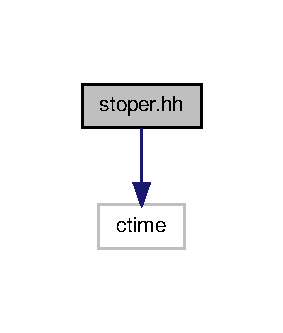
\includegraphics[width=136pt]{stoper_8hh__incl}
\end{center}
\end{figure}
\-Ten wykres pokazuje, które pliki bezpośrednio lub pośrednio załączają ten plik\-:\nopagebreak
\begin{figure}[H]
\begin{center}
\leavevmode
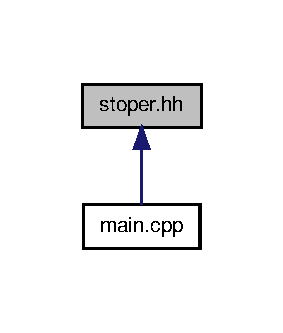
\includegraphics[width=136pt]{stoper_8hh__dep__incl}
\end{center}
\end{figure}
\subsection*{\-Komponenty}
\begin{DoxyCompactItemize}
\item 
class \hyperlink{classczas}{czas}
\end{DoxyCompactItemize}
\subsection*{\-Definicje}
\begin{DoxyCompactItemize}
\item 
\#define \hyperlink{stoper_8hh_a3d9fc3c745d0880902fe3ea3d5d5f71e}{\-C\-L\-O\-C\-K\-S\-\_\-\-P\-E\-R\-\_\-\-S\-E\-C}~1000000
\end{DoxyCompactItemize}


\subsection{\-Dokumentacja definicji}
\hypertarget{stoper_8hh_a3d9fc3c745d0880902fe3ea3d5d5f71e}{\index{stoper.\-hh@{stoper.\-hh}!\-C\-L\-O\-C\-K\-S\-\_\-\-P\-E\-R\-\_\-\-S\-E\-C@{\-C\-L\-O\-C\-K\-S\-\_\-\-P\-E\-R\-\_\-\-S\-E\-C}}
\index{\-C\-L\-O\-C\-K\-S\-\_\-\-P\-E\-R\-\_\-\-S\-E\-C@{\-C\-L\-O\-C\-K\-S\-\_\-\-P\-E\-R\-\_\-\-S\-E\-C}!stoper.hh@{stoper.\-hh}}
\subsubsection[{\-C\-L\-O\-C\-K\-S\-\_\-\-P\-E\-R\-\_\-\-S\-E\-C}]{\setlength{\rightskip}{0pt plus 5cm}\#define {\bf \-C\-L\-O\-C\-K\-S\-\_\-\-P\-E\-R\-\_\-\-S\-E\-C}~1000000}}\label{stoper_8hh_a3d9fc3c745d0880902fe3ea3d5d5f71e}


\-Definicja w linii 11 pliku stoper.\-hh.


\printindex
\end{document}
